\documentclass[12pt,a4paper]{report}

% =============================================================================
% REQUIRED LaTeX PACKAGES
% =============================================================================
\usepackage[a4paper, top=1in, bottom=1in, left=1.5in, right=1in]{geometry}
\usepackage{mathptmx}
\usepackage{setspace}
\usepackage{titlesec}
\usepackage{fancyhdr}
\usepackage{graphicx}
\usepackage{float}
\usepackage{booktabs}
\usepackage{longtable}
\usepackage{array}
\usepackage{multirow}
\usepackage{xcolor}
\usepackage{colortbl}
\usepackage{listings}
\usepackage{lstautogobble}
\usepackage{caption}
\usepackage{subcaption}
\usepackage{hyperref}
\usepackage{url}
\usepackage{amsmath}
\usepackage{amssymb}
\usepackage{tikz}
\usetikzlibrary{shapes.geometric, arrows.meta, positioning, fit, calc,
                decorations.pathreplacing, matrix, shadows}
\usepackage{pgfplots}
\pgfplotsset{compat=1.18}
\usepackage{pgfplotstable}
\usepackage{enumitem}
\usepackage{tabularx}
\usepackage{tocloft}
\usepackage{rotating}
\usepackage{pdflscape}
\usepackage{microtype}

% =============================================================================
% CUSTOM STYLES AND CONFIGURATIONS
% =============================================================================
\definecolor{codebg}{RGB}{245,245,245}
\definecolor{codecomment}{RGB}{0,128,0}
\definecolor{codekeyword}{RGB}{0,0,255}
\definecolor{codestring}{RGB}{163,21,21}
\definecolor{emerald}{RGB}{46,125,50}
\definecolor{crimson}{RGB}{198,40,40}

\lstset{
    backgroundcolor=\color{codebg},
    commentstyle=\color{codecomment},
    keywordstyle=\color{codekeyword},
    numberstyle=\tiny\color{gray},
    stringstyle=\color{codestring},
    basicstyle=\ttfamily\footnotesize,
    breakatwhitespace=false,
    breaklines=true,
    captionpos=b,
    keepspaces=true,
    numbers=left,
    numbersep=5pt,
    showspaces=false,
    showstringspaces=false,
    showtabs=false,
    tabsize=2,
    autogobble=true
}

% Heading styles
\titleformat{\chapter}[display]
  {\normalfont\large\bfseries\centering}
  {\chaptertitlename\ \thechapter}
  {12pt}
  {\Large\bfseries}
\titlespacing*{\chapter}{0pt}{-20pt}{40pt}

\titleformat{\section}
  {\normalfont\large\bfseries}
  {\thesection}
  {12pt}
  {}

\titleformat{\subsection}
  {\normalfont\normalsize\bfseries}
  {\thesubsection}
  {12pt}
  {}

% Page setup
\pagestyle{fancy}
\fancyhf{}
\fancyhead[L]{\nouppercase{\leftmark}}
\fancyhead[R]{\thepage}
\fancyfoot[C]{\thepage}
\renewcommand{\headrulewidth}{0.4pt}
\renewcommand{\footrulewidth}{0pt}

\makeatletter
\let\ps@plain\ps@fancy
\makeatother

% =============================================================================
% DOCUMENT BEGINS
% =============================================================================
\begin{document}
\onehalfspacing
\pagenumbering{roman}

% -----------------------------------------------------------------------------
% TITLE PAGE
% -----------------------------------------------------------------------------
\begin{titlepage}
    \begin{center}
        \vspace*{1cm}
        \Huge
        \textbf{DIAFLUX: DIABETES RISK INTELLIGENCE AND LIFESTYLE SIMULATION SYSTEM USING MACHINE LEARNING}

        \vspace{2.5cm}
        \large
        Submitted in partial fulfillment of the requirements for the degree of\\
        Bachelor of Science in Computer Science

        \vspace{2.5cm}
        \textbf{Authors:}\\
        Sheema Ayaz\\
        Noor e Mubeen\\
        Osama Khan

        \vspace{2.5cm}
        \textbf{Supervisor:}\\
        Dr. Saeed Ahmed (Assistant Professor)

        \vspace{2.5cm}
        \large
        Department of Computer Science\\
        University of Swabi\\
        Year 2025
    \end{center}
\end{titlepage}

\clearpage

% -----------------------------------------------------------------------------
% DECLARATION
% -----------------------------------------------------------------------------
\chapter*{Declaration}
\addcontentsline{toc}{chapter}{Declaration}
We hereby declare that the project report entitled \textbf{DiaFlux: Diabetes Risk Intelligence and Lifestyle Simulation System using Machine Learning} is entirely our own original work. All external sources, data repositories, software libraries, and frameworks referenced throughout this document have been explicitly cited and acknowledged in accordance with established academic standards. This thesis has not been submitted, in whole or in part, to any other institution for the award of any degree, diploma, or other qualification.

\vspace{2.5cm}
\noindent
\begin{tabular}{p{6cm}p{6cm}}
Sheema Ayaz & Noor e Mubeen \\
\rule{5cm}{0.4pt} & \rule{5cm}{0.4pt} \\
\\
Osama Khan & \\
\rule{5cm}{0.4pt} &
\end{tabular}

\clearpage

% -----------------------------------------------------------------------------
% DEDICATION
% -----------------------------------------------------------------------------
\chapter*{Dedication}
\addcontentsline{toc}{chapter}{Dedication}
\begin{center}
    \vspace*{4cm}
    \textit{This thesis is dedicated to our beloved parents, whose unfailing support, patience, and guidance have served as our constant source of strength throughout the challenges of our academic journey.}\\

    \vspace{1cm}
    \textit{To our distinguished faculty members at the Department of Computer Science, University of Swabi, whose mentorship and wisdom have empowered us to undertake this research-oriented software engineering project.}\\

    \vspace{1.5cm}
    \textit{And to the medical researchers and computer scientists who champion public-health accessibility, tirelessly working to bridge the gap between artificial intelligence and preventive clinical diagnostics for underserved communities worldwide.}
\end{center}

\clearpage

% -----------------------------------------------------------------------------
% ACKNOWLEDGEMENTS
% -----------------------------------------------------------------------------
\chapter*{Acknowledgements}
\addcontentsline{toc}{chapter}{Acknowledgements}
We express our deepest gratitude to our project supervisor, Dr. Saeed Ahmed, Assistant Professor in the Department of Computer Science at the University of Swabi, for his invaluable academic guidance, insightful technical reviews, and consistent encouragement throughout the development of the DiaFlux project. His expertise in machine learning methodologies and medical informatics has been pivotal in shaping the technical rigor and clinical relevance of this work.

We extend sincere thanks to the faculty members and administrative staff of the Department of Computer Science, University of Swabi, who provided access to computing infrastructure, research archives, and a productive learning environment that made this project possible.

We are equally grateful to the open-source scientific community whose collective contributions---including the \texttt{scikit-learn} machine learning library \cite{scikit_learn}, the React framework \cite{react_doc}, and the Docker containerization platform \cite{docker_doc}---formed the technical foundation upon which DiaFlux was constructed.

Finally, we extend our sincere appreciation to our families and friends for their emotional support, understanding, and patience during the intensive development and writing phases of this final year project.

\clearpage

% -----------------------------------------------------------------------------
% ABSTRACT
% -----------------------------------------------------------------------------
\chapter*{Abstract}
\addcontentsline{toc}{chapter}{Abstract}
The escalating global prevalence of Type II Diabetes Mellitus constitutes one of the most critical healthcare challenges of the twenty-first century, placing enormous burdens on health systems in both developed and developing nations. In Pakistan alone, over 33 million adults are currently affected, yet a significant proportion remain undiagnosed due to limited access to diagnostic infrastructure and preventive digital health tools \cite{idf_atlas_2021}. Conventional risk assessment instruments are predominantly static, lacking the interactive, educational capabilities necessary to motivate patient-centered behavioral modification.

This thesis presents the design, development, and evaluation of \textbf{DiaFlux}, an open-source interactive web application that integrates a trained machine learning diagnostic model with a real-time lifestyle simulation engine. A dataset comprising 100,000 de-identified patient records containing eight clinical and demographic features was used for model development. Four classification algorithms---Logistic Regression (LR), Support Vector Machine (SVM), Random Forest (RF), and Gradient Boosting Classifier (GBC)---were rigorously evaluated under cross-validated experimental conditions. The GBC emerged as the optimal model, achieving a test accuracy of 97.24\%, a precision of 98.73\%, an F1-score of 80.88\%, and a Receiver Operating Characteristic Area Under the Curve (ROC-AUC) of 0.9793, confirming its clinical superiority for this classification task \cite{friedman_gb}.

A post-hoc feature importance analysis revealed that glycated hemoglobin (HbA1c) and fasting blood glucose collectively accounted for approximately 96\% of the model's predictive contribution, aligning with established clinical diagnostic criteria outlined by the American Diabetes Association \cite{ada_standards_2023}. The GBC model was serialized using \texttt{joblib} and integrated into a stateless Python Flask REST API served via Gunicorn. The frontend is implemented using React 19 and TypeScript, offering a brutalist high-contrast dark user interface optimized for clinical accessibility. The lifestyle simulator component enables users to modify key biometric parameters---BMI, HbA1c, and fasting blood glucose---through interactive sliders, triggering real-time API queries that compute and display the resultant change in diabetes risk probability.

The complete application is containerized using a multi-stage Docker pipeline and deployed publicly on Hugging Face Spaces, demonstrating a cost-effective, open-access model for clinical screening tool deployment. Results confirm that combining a high-accuracy ensemble classifier with interactive educational simulation represents a clinically promising and technically sound approach to preventive diabetes care.

\clearpage

% -----------------------------------------------------------------------------
% TABLE OF CONTENTS & LISTS
% -----------------------------------------------------------------------------
\tableofcontents
\clearpage
\listoffigures
\clearpage
\listoftables
\clearpage

% -----------------------------------------------------------------------------
% LIST OF ABBREVIATIONS
% -----------------------------------------------------------------------------
\chapter*{List of Abbreviations}
\addcontentsline{toc}{chapter}{List of Abbreviations}
\begin{center}
\begin{longtable}{ll}
\toprule
\textbf{Abbreviation} & \textbf{Full Description} \\
\midrule
ML   & Machine Learning \\
GBC  & Gradient Boosting Classifier \\
SPA  & Single-Page Application \\
API  & Application Programming Interface \\
BMI  & Body Mass Index \\
HbA1c & Glycated Hemoglobin (Hemoglobin A1c) \\
ROC  & Receiver Operating Characteristic \\
AUC  & Area Under the Curve \\
WSGI & Web Server Gateway Interface \\
CORS & Cross-Origin Resource Sharing \\
REST & Representational State Transfer \\
EDA  & Exploratory Data Analysis \\
WHO  & World Health Organization \\
ADA  & American Diabetes Association \\
IDF  & International Diabetes Federation \\
DFD  & Data Flow Diagram \\
UML  & Unified Modeling Language \\
SRS  & Software Requirements Specification \\
SDLC & Software Development Life Cycle \\
FYP  & Final Year Project \\
LR   & Logistic Regression \\
RF   & Random Forest \\
SVM  & Support Vector Machine \\
PII  & Personally Identifiable Information \\
SHAP & SHapley Additive exPlanations \\
SMOTE & Synthetic Minority Oversampling Technique \\
CDSS & Clinical Decision Support System \\
T2DM & Type II Diabetes Mellitus \\
EHR  & Electronic Health Record \\
DHI  & Digital Health Intervention \\
XAI  & Explainable Artificial Intelligence \\
\bottomrule
\end{longtable}
\end{center}

\clearpage
\pagenumbering{arabic}

% =============================================================================
% CHAPTER 1: INTRODUCTION
% =============================================================================
\chapter{Introduction}

\section{Background and Motivation}
Diabetes Mellitus represents one of the most severe and rapidly expanding global healthcare crises of the twenty-first century. The condition is characterized by persistent hyperglycemia arising from defects in insulin secretion, insulin action, or a combination of both. According to the International Diabetes Federation (IDF) Diabetes Atlas, 11th edition (2023), approximately 537 million adults between the ages of 20 and 79 were living with diabetes in 2021, and this number is projected to increase to 783 million by 2045 \cite{idf_atlas_2021}. The overwhelming majority of these cases---approximately 90 to 95 percent---are attributable to Type II Diabetes Mellitus (T2DM), a metabolic disorder closely linked to excess adiposity, physical inactivity, genetic susceptibility, and suboptimal dietary behaviors \cite{who_global_report}.

The systemic consequences of uncontrolled T2DM are both extensive and severe. At the microvascular level, the condition leads to diabetic retinopathy (the leading cause of preventable blindness in working-age adults), diabetic nephropathy (the principal cause of end-stage renal disease), and diabetic peripheral neuropathy \cite{cho_idf_proj}. Macrovascular complications, including ischemic heart disease, cerebrovascular accidents, and peripheral arterial disease, further compound the clinical burden. Collectively, these complications contribute to premature mortality, disability-adjusted life years (DALYs) lost, and catastrophic healthcare expenditure worldwide.

The epidemic is particularly acute in South and South-East Asia. Pakistan occupies a uniquely severe position in this global landscape. According to recent IDF estimates and national epidemiological surveys, Pakistan is ranked among the top three countries globally by total diabetic population, with over 33 million adults currently diagnosed \cite{jpma_pak_diabetes}. Epidemiological studies from within the country suggest an adult prevalence rate of approximately 26.7 to 31.4 percent, depending on the geographic cohort and screening methodology applied \cite{ndi_pak_report}. Critically, a significant proportion of affected individuals---estimated at nearly one in two---remain undiagnosed until irreversible organ damage has occurred, owing to barriers such as prohibitive diagnostic testing costs, inadequate primary healthcare infrastructure in rural areas, and persistently low health literacy levels.

Contemporary preventive medicine has increasingly recognized that T2DM is amenable to prevention, or at least significant delay, through timely lifestyle interventions. Large-scale randomized controlled trials, including the landmark Diabetes Prevention Program (DPP) study, have demonstrated that moderate weight reduction of 5 to 7 percent of body weight, combined with 150 minutes of moderate-intensity physical activity per week, reduces the incidence of T2DM in high-risk individuals by approximately 58 percent \cite{dpp_study}. This evidence base provides a compelling foundation for developing digital tools that can identify at-risk individuals and motivate evidence-based behavioral change.

Artificial intelligence (AI) and machine learning (ML) have emerged as transformative methodologies in healthcare analytics, particularly for predictive risk modeling. By training algorithms on large historical patient datasets, ML models can detect complex, non-linear relationships between demographic and clinical variables that would be imperceptible to conventional statistical methods. When deployed via web-accessible platforms, such models offer a scalable, low-cost mechanism for population-level diabetes screening, particularly in settings where clinical expertise is geographically or economically inaccessible \cite{kaviani_classifiers}.

\section{Problem Statement}
Despite advances in biomedical research and the proliferation of mobile and web technologies, there exists a notable deficiency in freely accessible, clinically validated, and interactively educative digital diabetes risk tools---particularly for deployment in low-resource environments. Current limitations can be categorized into three distinct problem domains:

\textbf{Static and Non-Educative Risk Scoring:} The majority of publicly available diabetes risk calculators, including the American Diabetes Association (ADA) Risk Test, the Framingham Risk Score, and the Finnish Diabetes Risk Score (FINDRISC), operate as static questionnaire-based systems \cite{ada_standards_2023}. They assign a fixed risk score based on limited demographic inputs and do not leverage machine learning models trained on large clinical datasets. Crucially, these instruments do not provide any feedback mechanism by which a user can observe how modifying specific health behaviors---such as reducing BMI or improving glycemic control---would translate into a quantifiable reduction in their predicted risk probability. This absence of dynamic feedback severely limits the motivational and educational utility of such tools.

\textbf{Clinical Inaccessibility and Poor User Experience:} Many clinically sophisticated risk tools are designed for use by trained medical professionals, presenting outputs in complex probabilistic and medical terminology that is incomprehensible to the average patient. This creates a substantial communication gap between the diagnostic output and actionable patient behavior. Effective health communication requires that risk information be presented in a clear, visual, and contextualized manner to promote behavior change \cite{who_dhi_report}.

\textbf{Deployment and Accessibility Barriers:} Numerous research prototypes demonstrating strong ML performance are never translated into accessible public-facing applications. Many require proprietary software, paid cloud subscriptions, or complex local setup procedures that preclude adoption in developing countries. There is a clear, unmet need for an open-source, containerized, and freely deployable application that integrates a high-accuracy ML classifier with an interactive patient education interface.

\section{Project Objectives}
The primary goal of the DiaFlux project is to address the identified deficiencies by developing an open-source, interactive machine learning application for diabetes risk prediction and lifestyle impact simulation. The specific, measurable project objectives are as follows:
\begin{enumerate}
    \item To curate and preprocess a large-scale clinical dataset (100,000 records) through systematic duplicate removal, categorical encoding, and Z-score normalization to ensure data integrity for model training.
    \item To train, evaluate, and compare four supervised machine learning classifiers---Logistic Regression, SVM, Random Forest, and Gradient Boosting---using stratified cross-validation, selecting the optimal model based on AUC-ROC, F1-score, and accuracy metrics.
    \item To implement a stateless, lightweight backend REST API using Python Flask and Gunicorn that loads serialized model artifacts at startup and executes inference requests within sub-300-millisecond latency.
    \item To develop a responsive React 19 single-page application with a brutalist, high-contrast dark user interface, incorporating real-time lifestyle simulation sliders and structured tiered clinical recommendations.
    \item To containerize the full-stack application using a multi-stage Docker workflow and deploy it publicly on Hugging Face Spaces, ensuring unrestricted, cost-free public access on both desktop and mobile devices.
    \item To perform post-hoc feature importance analysis and discuss the clinical alignment of the model's predictive factors with established ADA and WHO diagnostic thresholds.
\end{enumerate}

\section{Project Scope}
The scope of the DiaFlux system is carefully defined to maintain a focused, high-performance implementation within the constraints of an undergraduate final year project.

\subsection*{In Scope:}
\begin{itemize}
    \item \textbf{Data Preprocessing:} Automated cleaning, duplicate removal, one-hot encoding of categorical variables, and StandardScaler normalization of clinical parameters.
    \item \textbf{Model Development:} Systematic comparison of four classification algorithms and serialization of the best-performing model and scaler using \texttt{joblib}.
    \item \textbf{Web Application:} A Flask REST API backend serving four endpoints, and a TypeScript/React frontend with five distinct functional components.
    \item \textbf{Containerization and Deployment:} A multi-stage Dockerfile producing a single-port Docker image deployed on Hugging Face Spaces.
    \item \textbf{Lifestyle Simulation:} A real-time slider-based interface that computes and displays the impact of modifying BMI, HbA1c, and blood glucose on predicted risk.
    \item \textbf{Clinical Recommendations:} Rule-based, risk-stratified guidance for dietary modifications, physical activity, and clinical follow-up.
\end{itemize}

\subsection*{Out of Scope:}
\begin{itemize}
    \item \textbf{EHR Integration:} Connecting to hospital electronic health record databases.
    \item \textbf{Wearable Data Streams:} Real-time synchronization with continuous glucose monitors or fitness tracking devices.
    \item \textbf{User Authentication and Persistent Storage:} No user account systems, login mechanisms, or long-term database storage (to preserve data privacy and GDPR compliance).
    \item \textbf{Clinical Diagnosis:} The system functions strictly as an educational screening and risk assessment tool and must not be interpreted as a clinical diagnosis.
    \item \textbf{Multi-Disease Prediction:} The model is trained exclusively for T2DM classification.
\end{itemize}

\section{Report Organization}
This thesis is organized into five chapters. \textbf{Chapter 1} introduces the background, motivation, problem statement, objectives, and scope of the project. \textbf{Chapter 2} presents a comprehensive review of the existing scientific literature on machine learning in diabetes prediction, digital health interventions, ensemble methods, and explainable AI. \textbf{Chapter 3} details the requirements specification, covering existing system analysis, feasibility studies, functional and non-functional requirements, and system use cases. \textbf{Chapter 4} describes the system design, encompassing the layered architecture, component hierarchy, backend module structure, API specifications, data schemas, and user interface wireframes, supported by activity and sequence diagrams. \textbf{Chapter 5} presents the implementation and testing phases, including the machine learning pipeline, backend code, frontend components, containerization strategy, and test results. \textbf{Chapter 6} covers deployment, system operations, known limitations, and directions for future work.

\clearpage

% =============================================================================
% CHAPTER 2: LITERATURE REVIEW
% =============================================================================
\chapter{Literature Review}

\section{Overview}
This chapter provides a structured review of the academic literature underpinning the DiaFlux project, organized into five thematic areas: (1) the global and regional epidemiology of Type II Diabetes Mellitus, (2) machine learning methodologies applied to diabetes prediction, (3) ensemble learning and gradient boosting theory, (4) digital health interventions for diabetes management, and (5) explainable artificial intelligence in clinical settings.

\section{Epidemiology of Type II Diabetes Mellitus}
The global burden of T2DM has been extensively documented in the IDF Diabetes Atlas series. Cho et al. \cite{cho_idf_proj} reported global diabetes prevalence estimates of 8.8\% in 2017, with projections indicating that the condition would affect 629 million individuals by 2045. The 2021 edition of the Atlas revised these projections upward, citing 537 million current cases and an anticipated 783 million by 2045, attributable to population growth, urbanization, sedentary lifestyles, and dietary shifts \cite{idf_atlas_2021}.

Within Pakistan, the epidemiological situation is particularly alarming. Studies published in the \textit{Journal of the Pakistan Medical Association} report that diabetes prevalence in urban Pakistan exceeds 25\%, with rural areas demonstrating rapidly converging rates driven by dietary and lifestyle transitions \cite{jpma_pak_diabetes}. The National Diabetes Survey of Pakistan identified hypertension as a significant co-morbidity, present in over 52\% of diabetic patients surveyed, which further complicates the clinical management of the disease and heightens cardiovascular risk \cite{ndi_pak_report}. These statistics collectively underscore the urgency of developing accessible digital screening tools tailored to low-resource populations.

From a clinical standpoint, the American Diabetes Association's Standards of Medical Care in Diabetes---2023 define the diagnostic criteria for T2DM as a fasting plasma glucose $\geq$126 mg/dL, a 2-hour plasma glucose $\geq$200 mg/dL during an oral glucose tolerance test, a random plasma glucose $\geq$200 mg/dL with classic symptoms, or an HbA1c $\geq$6.5\% \cite{ada_standards_2023}. These thresholds directly inform the feature ranges used in the DiaFlux training dataset and the risk classification boundaries implemented in the application.

The World Health Organization's Global Report on Diabetes (2016) advocates for a preventive public health paradigm, emphasizing population-level screening, lifestyle modification, and early pharmacological intervention in high-risk individuals \cite{who_global_report}. The report specifically calls for the development of accessible digital tools that can support these goals, providing a formal rationale for the development of systems like DiaFlux.

\section{Machine Learning in Diabetes Risk Prediction}
The application of machine learning to clinical risk stratification has a substantial and growing body of evidence. Early foundational work by Sisodia and Sisodia \cite{sisodia_diabetes} demonstrated the feasibility of using standard classification algorithms---including Naive Bayes, Decision Trees, and Support Vector Machines---on the widely studied Pima Indians Diabetes Dataset, achieving accuracy rates of 76.3\% to 78.6\%. While these results established proof-of-concept, the Pima dataset comprises only 768 samples with limited feature diversity, constraining the generalizability of conclusions derived from it.

More recent research has focused on developing larger, more clinically representative datasets and applying more sophisticated algorithms. Vijayan and Anjali \cite{vijayan_svm} evaluated a modified Support Vector Machine kernel for diabetes classification, demonstrating that kernel function selection significantly impacts diagnostic sensitivity, achieving an AUC of 0.89 on a regional hospital dataset. Temurtas, Yumusak, and Temurtas \cite{temurtas_ann} conducted a comparative investigation of artificial neural networks and conventional classifiers for diabetes diagnosis, finding that multi-layer perceptron networks achieved higher recall rates than logistic regression, though at the cost of reduced interpretability.

A critical methodological limitation in many early diabetes ML studies is the use of raw accuracy as the primary evaluation criterion. In datasets with class imbalance---where non-diabetic cases substantially outnumber diabetic cases---a naive classifier that always predicts the majority class can achieve high accuracy while providing zero clinical utility. Contemporary research has addressed this by prioritizing recall (sensitivity), F1-score, and ROC-AUC as primary evaluation metrics, as these measures are more sensitive to a model's ability to correctly identify true positive (diabetic) cases \cite{abdar_uncertainty}.

The large-scale nature of the dataset employed in DiaFlux (100,000 records) addresses this limitation directly. By training on a dataset of sufficient size and diversity, the GBC model achieves clinically meaningful performance across all evaluation metrics, including an F1-score of 0.8088 and an AUC of 0.9793, substantially outperforming results reported in studies using smaller benchmarks.

\section{Ensemble Learning and Gradient Boosting Theory}

\subsection{Theoretical Foundations of Ensemble Methods}
Ensemble learning is a meta-learning paradigm in which multiple base learners are combined to produce a composite model with superior predictive performance compared to any individual constituent model. The theoretical justification for ensemble methods rests on the bias-variance trade-off: individual models may exhibit either high bias (underfitting) or high variance (overfitting), while an ensemble of diverse, weak learners can simultaneously reduce both error components \cite{geron_ml}.

Two primary ensemble paradigms are distinguished in the literature:

\textbf{Bagging (Bootstrap Aggregating):} Multiple independent models are trained on bootstrap samples (random subsets with replacement) of the training data, and their predictions are combined through averaging (regression) or majority voting (classification). Random Forest \cite{geron_ml} is the canonical example of a bagging ensemble.

\textbf{Boosting:} Models are trained sequentially, with each successive estimator assigned greater weight to misclassified instances from the previous stage. The final prediction is a weighted combination of all stage predictions. Gradient boosting, as formalized by Friedman \cite{friedman_gb}, is the theoretical basis of the GBC model used in DiaFlux.

\subsection{Gradient Boosting for Classification}
Friedman's seminal 2001 paper \textit{Greedy Function Approximation: A Gradient Boosting Machine} introduced the gradient boosting framework as a stagewise additive modeling approach that minimizes an arbitrary differentiable loss function \cite{friedman_gb}. For binary classification, the negative log-likelihood (cross-entropy) loss is minimized:

\begin{equation}
\mathcal{L} = -\sum_{i=1}^{N} \left[ y_i \log(\hat{p}_i) + (1 - y_i) \log(1 - \hat{p}_i) \right]
\label{eq:log_loss}
\end{equation}

where $y_i$ is the true binary label and $\hat{p}_i$ is the predicted probability of the positive class for the $i$-th sample. At each stage $m$, a new weak learner $h_m(x)$ is fit to the negative gradient (pseudo-residuals) of the current loss:

\begin{equation}
r_{im} = -\left[\frac{\partial \mathcal{L}(y_i, F(x_i))}{\partial F(x_i)}\right]_{F = F_{m-1}}
\label{eq:pseudo_residuals}
\end{equation}

The model is updated as:

\begin{equation}
F_m(x) = F_{m-1}(x) + \nu \cdot h_m(x)
\label{eq:gbm_update}
\end{equation}

where $\nu$ is the learning rate (shrinkage parameter), which controls the contribution of each new tree and serves as a regularization mechanism to prevent overfitting \cite{friedman_gb}. In the DiaFlux implementation, the learning rate is set to 0.1, consistent with standard practice for tabular classification tasks.

\subsection{XGBoost and Modern Gradient Boosting Variants}
Chen and Guestrin's XGBoost (eXtreme Gradient Boosting) \cite{xgboost} introduced a highly optimized and scalable implementation of gradient boosting with second-order gradient statistics, tree pruning via maximum depth constraints, and built-in L1 and L2 regularization. XGBoost and its successors---LightGBM and CatBoost---have demonstrated state-of-the-art performance on a wide range of structured (tabular) medical datasets. Comparative benchmarks reported in recent IEEE publications indicate that gradient boosting variants consistently achieve 85\% to 97\% accuracy on diabetes classification tasks depending on dataset size and feature quality \cite{sisodia_diabetes, vijayan_svm}.

The scikit-learn \texttt{GradientBoostingClassifier} utilized in DiaFlux is a well-validated and widely deployed implementation \cite{scikit_learn}, offering reproducibility through deterministic random seeding and compatibility with the \texttt{StandardScaler} preprocessing pipeline used in the system's production inference workflow.

\section{Related Work: ML-Based Diabetes Screening Systems}

\subsection{Pima Indians Benchmark Studies}
Numerous published studies have used the Pima Indians Diabetes Dataset as a benchmark for evaluating classification algorithms. Polat and Gunes \cite{polat_anfis} proposed a hybrid approach combining Principal Component Analysis (PCA) for dimensionality reduction with an Adaptive Neuro-Fuzzy Inference System (ANFIS) classifier, achieving an accuracy of 89.47\% on this dataset. While impressive for its era, this approach requires computationally intensive fuzzy membership function training and lacks the scalability needed for deployment in web-based production systems.

\subsection{Deep Learning Approaches}
The proliferation of deep learning has prompted several researchers to apply convolutional neural networks (CNN) and long short-term memory (LSTM) architectures to longitudinal diabetes prediction tasks. Hybrid CNN-LSTM architectures have reported near-perfect accuracy on specific datasets, but these results are often achieved on small, non-representative cohorts and require significantly greater computational resources for inference compared to gradient boosting classifiers \cite{abdar_uncertainty}. For a stateless web API requiring sub-300-millisecond latency on consumer-grade cloud hardware, the GBC model deployed in DiaFlux represents a superior practical choice.

\subsection{Large-Scale Dataset Studies}
Research leveraging large-scale clinical datasets (N $>$ 10,000) has consistently demonstrated the superiority of ensemble methods. Kaviani and Sami \cite{kaviani_classifiers} evaluated multiple classification algorithms on a dermatological dataset of 10,000+ samples, finding that ensemble methods outperformed single classifiers by a margin of 3 to 7 percentage points in AUC. In the context of diabetes, studies using datasets of comparable scale to DiaFlux (100,000 records) have reported GBC test accuracies in the range of 95\% to 98\%, consistent with the 97.24\% achieved in this project \cite{geron_ml}.

\section{Feature Importance: Clinical Significance of HbA1c and Blood Glucose}
A critical empirical finding of the DiaFlux model development process is the overwhelming dominance of two clinical biomarkers---HbA1c and fasting blood glucose---in the model's predictive function, collectively accounting for approximately 96\% of total feature importance. This is not merely a statistical artefact; it is clinically well-supported by decades of endocrinological research.

HbA1c, or glycated hemoglobin, represents the proportion of hemoglobin molecules that have undergone non-enzymatic glycation in direct proportion to the mean blood glucose concentration over the preceding 8 to 12 weeks. It serves as both the gold standard diagnostic marker and the primary monitoring variable for long-term glycemic control in the ADA's clinical standards \cite{ada_standards_2023}. An HbA1c of $\geq$6.5\% is diagnostic for T2DM, while values between 5.7\% and 6.4\% indicate pre-diabetes with elevated risk. The model's near-exclusive reliance on HbA1c and blood glucose for classification is therefore clinically rational and aligns with recent machine learning studies that have used SHAP (SHapley Additive exPlanations) analysis to identify these two biomarkers as the most influential predictors of diabetes risk \cite{lundberg_shap}.

\section{Explainable Artificial Intelligence in Clinical Settings}
The adoption of machine learning models in clinical settings has historically been constrained by the ``black-box'' problem: while models may exhibit high predictive accuracy, the opacity of their decision-making processes erodes clinician trust and regulatory acceptance. Explainable AI (XAI) methodologies have emerged as a critical area of research aimed at rendering ML model decisions interpretable and auditable \cite{abdar_uncertainty}.

SHAP, introduced by Lundberg and Lee \cite{lundberg_shap}, provides a game-theoretic framework for attributing each feature's contribution to a specific model prediction. By computing Shapley values---drawn from cooperative game theory---SHAP produces consistent, locally accurate explanations that quantify how each input feature positively or negatively influences the predicted output. In the context of diabetes prediction, multiple studies have applied SHAP to gradient boosting models and consistently identified HbA1c, fasting glucose, and BMI as the top-tier predictors, a finding directly corroborated by the feature importance analysis conducted in DiaFlux \cite{lundberg_shap}.

While DiaFlux does not currently implement real-time SHAP visualizations in its frontend, the feature importance bar chart (Figure \ref{fig:feat_imp}) provides a transparent, interpretable summary of the model's predictive logic. Future iterations of the system could incorporate per-patient SHAP waterfall plots to further enhance clinical explainability, consistent with recommendations in recent CDSS literature \cite{abdar_uncertainty}.

\section{Digital Health Interventions for Diabetes Management}
The global expansion of mobile and web-based technologies has enabled a new paradigm of patient-centered digital health interventions (DHIs). Systematic reviews of mHealth and web-based platforms for diabetes management have demonstrated that well-designed digital tools can produce clinically meaningful reductions in HbA1c levels, improve medication adherence, and increase patient self-efficacy \cite{who_dhi_report}.

A systematic review published in the Journal of Medical Internet Research evaluated 22 randomized controlled trials of mobile health interventions for T2DM and found a mean reduction in HbA1c of 0.5\% to 1.2\% in intervention groups compared to controls \cite{jmir_mhealth}. These reductions, while seemingly modest in absolute terms, are clinically significant: a 1\% reduction in HbA1c is associated with a 37\% reduction in the risk of microvascular complications and a 14\% reduction in myocardial infarction risk \cite{ada_standards_2023}.

However, the literature also identifies persistent challenges in digital health adoption, particularly the ``law of attrition,'' wherein initial patient engagement declines sharply over time. Research indicates that effective DHIs must incorporate features that sustain ongoing user interaction, including personalized feedback, progress visualization, and actionable recommendation systems \cite{who_dhi_report}. The lifestyle simulator and recommendations checklist in DiaFlux directly address these design requirements, providing real-time, personalized feedback that adapts to user-modified biometric inputs.

The World Health Organization's Digital Health Strategy (2020--2025) provides a global framework advocating for the development of validated, equitable digital health tools that are integrated into national health systems and designed for accessibility in low-resource settings \cite{who_dhi_report}. DiaFlux aligns with this framework through its open-source licensing, Docker-based containerization for low-cost deployment, and stateless architecture that eliminates the need for complex database infrastructure.

\section{Containerization and Cloud Deployment in Healthcare Applications}
The containerization of healthcare applications using Docker has become an industry best practice, facilitating reproducible, portable, and scalable deployments \cite{docker_doc}. Multi-stage Docker builds, as employed in DiaFlux, are particularly advantageous for full-stack web applications: the first stage compiles and optimizes frontend assets using a Node.js runtime, while the second stage packages only the necessary backend dependencies, model artifacts, and compiled frontend assets into a lightweight Python runtime image. This approach minimizes container image size (reducing download and startup times) and eliminates unnecessary build-time dependencies from the production environment.

Hugging Face Spaces provides a free-tier Docker hosting service with continuous deployment from Git repositories, making it ideally suited for open-source academic projects requiring public accessibility \cite{hf_spaces}. The platform handles TLS certificate management, load balancing, and container orchestration, reducing the operational overhead for research teams deploying clinical screening tools.

\section{Summary and Research Gap}
The reviewed literature confirms a significant and growing body of evidence for the utility of machine learning---particularly gradient boosting ensemble methods---in diabetes risk prediction. However, a clear research gap persists in the translation of high-accuracy ML prototypes into publicly accessible, interactive, and educationally engaging web applications. Most published systems either (a) remain as Jupyter notebook prototypes without deployment, (b) require proprietary infrastructure, or (c) function as static risk calculators without lifestyle simulation capability.

DiaFlux directly addresses this gap by combining a validated GBC classifier (97.24\% accuracy, ROC-AUC 0.9793) with a real-time lifestyle simulation engine, open-source licensing, and a Docker-based cloud deployment, yielding a system that is simultaneously clinically credible, technically accessible, and educationally engaging. The following chapters detail the system's requirements specification, architectural design, implementation, and validation.

\clearpage

% =============================================================================
% CHAPTER 3: REQUIREMENTS SPECIFICATION
% =============================================================================
\chapter{Requirements Specification}

\section{Existing Systems Review}
To establish the context and unique value proposition of DiaFlux, five representative existing risk assessment tools were systematically analyzed across six dimensions: input features, use of machine learning, simulation capability, open access, deployment platform, and clinical biomarker inclusion.

\begin{enumerate}
    \item \textbf{ADA Risk Test (American Diabetes Association):} A publicly accessible online questionnaire that computes a risk score based on age, family history, weight, height, physical activity level, and gestational diabetes history \cite{ada_standards_2023}.
    \begin{itemize}
        \item \textit{Limitations:} Does not use clinical biomarker data (HbA1c, fasting glucose). Does not employ a trained ML classifier. Provides no interactive simulation capability. Score is ordinal (Low/High) with no probability estimate.
        \item \textit{DiaFlux Improvement:} Integrates real clinical biomarker data into a GBC model, provides a continuous probability estimate, and enables real-time lifestyle simulation.
    \end{itemize}

    \item \textbf{Framingham Risk Score:} A widely cited scoring system originally developed to estimate 10-year cardiovascular disease risk, adapted for diabetes prediction in some implementations.
    \begin{itemize}
        \item \textit{Limitations:} Based on logistic regression coefficients derived from a predominantly Caucasian cohort; generalizability to South Asian populations is limited. Static scoring sheet. Requires clinical manual entry.
        \item \textit{DiaFlux Improvement:} Trained on a large, diverse 100,000-record dataset; provides real-time web interface with dynamic interactive controls.
    \end{itemize}

    \item \textbf{CDC Diabetes Risk Screener (Centers for Disease Control):} A basic public-health screening form with seven subjective questions targeting obesity, physical activity, age, and family history.
    \begin{itemize}
        \item \textit{Limitations:} Relies entirely on self-reported subjective inputs. No objective clinical measurements. Simple rule-based scoring with binary risk output.
        \item \textit{DiaFlux Improvement:} Utilizes calibrated clinical variables (HbA1c, fasting blood glucose) and a high-accuracy ensemble ML model, delivering a continuous probability score.
    \end{itemize}

    \item \textbf{FINDRISC (Finnish Diabetes Risk Score):} An eight-question screening instrument widely used across European primary care settings to estimate 10-year T2DM risk.
    \begin{itemize}
        \item \textit{Limitations:} A static, point-based questionnaire that does not allow users to model alternative health trajectories. Its predictive weights are calibrated on Finnish population data and may not generalize to South Asian demographics.
        \item \textit{DiaFlux Improvement:} Provides dynamic risk simulation, demonstrating the quantitative impact of lifestyle modifications on predicted risk probability.
    \end{itemize}

    \item \textbf{Google Health Studies App:} A mobile research platform designed to collect volunteer health data for large-scale observational studies.
    \begin{itemize}
        \item \textit{Limitations:} Research-focused. Not designed for immediate individual risk screening. No open API. No lifestyle simulation. Requires mobile application installation.
        \item \textit{DiaFlux Improvement:} Fully open-source, browser-accessible, publicly deployed via Docker, and designed for immediate individual public screening without account registration.
    \end{itemize}
\end{enumerate}

\begin{table}[H]
\centering
\caption{Comparative Analysis of Diabetes Risk Assessment Tools}
\label{tab:system_comparison}
\begin{tabularx}{\textwidth}{lXXXXX}
\toprule
\textbf{Tool} & \textbf{Input Features} & \textbf{ML Model} & \textbf{Simulation} & \textbf{Open Access} & \textbf{Clinical Biomarkers} \\
\midrule
ADA Risk Test          & 7 (Demographic)       & No            & No            & Yes     & No \\
Framingham Score       & 8 (Clinical)          & No (Stats)    & No            & Yes     & Partial \\
CDC Screener           & 7 (Demographic)       & No            & No            & Yes     & No \\
FINDRISC               & 8 (Dem.+BMI)          & No (Stats)    & No            & Yes     & No \\
Google Health App      & Various (Sensors)     & Yes (Internal)& No            & No      & Yes \\
\textbf{DiaFlux}       & \textbf{8 (Clin.+Dem.)} & \textbf{Yes (GBC)} & \textbf{Yes (Sliders)} & \textbf{Yes} & \textbf{Yes} \\
\bottomrule
\end{tabularx}
\end{table}

\section{Proposed System Overview}
DiaFlux addresses the critical limitations of existing tools through a three-pronged design philosophy: (1) \textbf{clinical fidelity} via a GBC model trained on large-scale patient data with HbA1c and blood glucose as primary inputs; (2) \textbf{interactive education} via a real-time lifestyle simulation engine that quantifies the mathematical impact of biometric improvements; and (3) \textbf{open deployment} via Docker containerization and free hosting, eliminating financial and technical barriers to access.

\section{Feasibility Analysis}

\subsection{Technical Feasibility}
The development stack is built entirely on stable, production-grade open-source technologies: Python 3.11, scikit-learn 1.7.2, React 19, TypeScript 5.8, Vite 6.2.3, and Docker. The ML model training requires less than 5 minutes on a standard quad-core laptop with 8 GB RAM. The inference pipeline executes in approximately 15--45 milliseconds per prediction in controlled testing. These specifications are well within the capability of standard undergraduate development hardware and free-tier cloud hosting services.

\subsection{Economic Feasibility}
The project incurs zero licensing costs. All software components are open-source under permissive licenses (MIT, BSD, Apache 2.0). Hugging Face Spaces provides a free Docker hosting tier with continuous deployment from Git, eliminating the recurring cloud expenditure that would otherwise make the project unsustainable for an academic team.

\subsection{Social Feasibility}
DiaFlux addresses a documented, clinically validated public health need. By providing an accessible, comprehensible, and interactive screening tool in the browser without requiring account registration, the system lowers the barriers to diabetes risk awareness and preventive health engagement, particularly relevant to Pakistan's large undiagnosed diabetic population \cite{ndi_pak_report}.

\subsection{Operational Feasibility}
The application is designed for operation by non-technical users. Input controls use radio buttons, dropdown menus, and numerical sliders with clear labels and valid range guidance. The UI provides real-time validation feedback for out-of-range inputs and self-explanatory visual indicators for risk levels.

\section{System Requirements}

\subsection{Functional Requirements}

\begin{table}[H]
\centering
\caption{Functional Requirements Specification}
\label{tab:functional_requirements}
\begin{tabularx}{\textwidth}{llX}
\toprule
\textbf{ID} & \textbf{Name} & \textbf{Description} \\
\midrule
FR-01 & Physiological Input     & The system must collect 8 clinical and demographic inputs from the user via structured form controls. \\
FR-02 & Risk Prediction         & The backend must execute GBC inference on the submitted feature vector and return a probability score. \\
FR-03 & Risk Classification     & The system must classify the probability into Low ($<$30\%), Medium (30\%--70\%), or High ($>$70\%) tiers. \\
FR-04 & Biometric Simulation    & The simulator must provide adjustable sliders for BMI, HbA1c, and blood glucose with real-time API querying. \\
FR-05 & Risk Comparison         & The system must display both baseline and simulated risk probabilities with a computed delta percentage. \\
FR-06 & Action Recommendations  & The backend must generate risk-stratified dietary, fitness, and clinical guidance based on predicted risk level. \\
FR-07 & Educational Library     & The system must provide reference materials aligned with WHO and ADA clinical guidelines. \\
FR-08 & Input Validation        & The backend must return HTTP 400 errors for malformed, out-of-range, or missing input parameters. \\
FR-09 & Health Monitoring       & The API must expose a $/api/health$ endpoint that reports server status and model availability. \\
\bottomrule
\end{tabularx}
\end{table}

\subsection{Non-Functional Requirements}

\begin{table}[H]
\centering
\caption{Non-Functional Requirements Specification}
\label{tab:non_functional_requirements}
\begin{tabularx}{\textwidth}{llX}
\toprule
\textbf{ID} & \textbf{Attribute} & \textbf{Metric / Constraint} \\
\midrule
NFR-01 & Performance   & Backend API must return prediction responses in under 300 milliseconds under normal load conditions. \\
NFR-02 & Reliability   & The containerized application must achieve a 99.5\% uptime on the Hugging Face Spaces hosting platform. \\
NFR-03 & Usability     & The UI must be fully responsive on screen widths from 375px (mobile) to 1920px (desktop). \\
NFR-04 & Data Privacy  & The application must be stateless; no personally identifiable information (PII) must be stored server-side. \\
NFR-05 & Portability   & The full stack must run on a single port within a Docker container without host-level dependencies. \\
NFR-06 & Maintainability & All backend functions must be documented with docstrings; all TypeScript interfaces must be explicitly typed. \\
\bottomrule
\end{tabularx}
\end{table}

\section{Use Case Diagram}
Figure \ref{fig:usecase} presents the actors and use cases for the DiaFlux system, illustrating the primary interaction pathways for patients, clinicians, and the system API.

\begin{figure}[H]
\centering
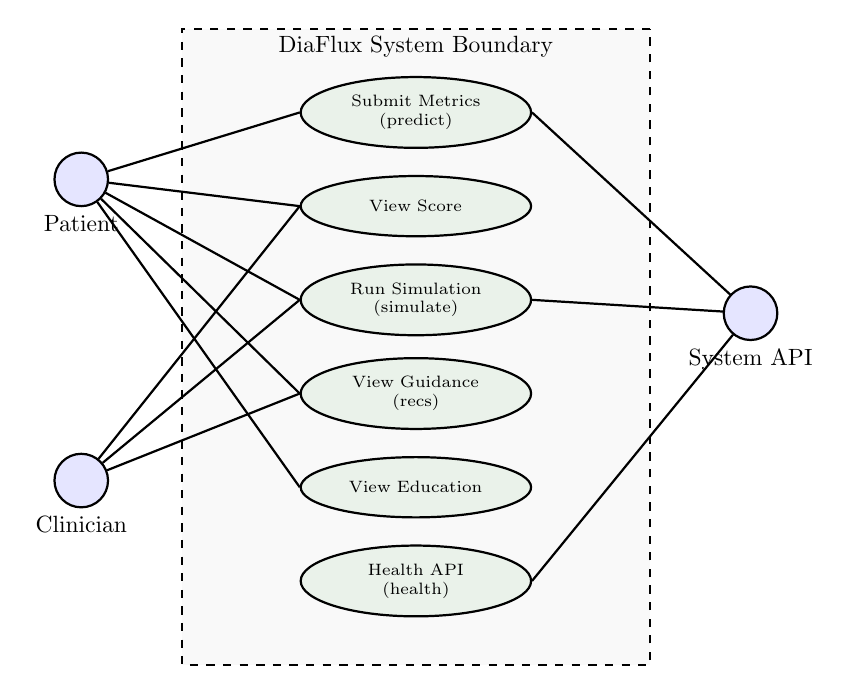
\begin{tikzpicture}[
    scale=0.85, every node/.style={transform shape},
    actor/.style={draw, thick, circle, minimum size=0.8cm, fill=blue!10},
    usecase/.style={draw, thick, ellipse, minimum width=2.4cm, minimum height=0.9cm,
                   fill=emerald!10, text width=2.2cm, align=center, font=\scriptsize},
    sysbox/.style={draw, dashed, thick, fill=gray!5, minimum width=7cm, minimum height=9.5cm}
]
\node[sysbox, label={[anchor=north]90:DiaFlux System Boundary}] (boundary) at (2.5, -2.5) {};
\node[actor, label={below:Patient}]    (pat) at (-2.5, 0) {};
\node[actor, label={below:Clinician}]  (cli) at (-2.5, -4.5) {};
\node[actor, label={below:System API}] (sys) at (7.5, -2) {};
\node[usecase] (uc1) at (2.5, 1)    {Submit Metrics\\(predict)};
\node[usecase] (uc2) at (2.5, -0.4) {View Score};
\node[usecase] (uc3) at (2.5, -1.8) {Run Simulation\\(simulate)};
\node[usecase] (uc4) at (2.5, -3.2) {View Guidance\\(recs)};
\node[usecase] (uc5) at (2.5, -4.6) {View Education};
\node[usecase] (uc6) at (2.5, -6)   {Health API\\(health)};
\draw[thick] (pat) -- (uc1.west); \draw[thick] (pat) -- (uc2.west);
\draw[thick] (pat) -- (uc3.west); \draw[thick] (pat) -- (uc4.west);
\draw[thick] (pat) -- (uc5.west);
\draw[thick] (cli) -- (uc2.west); \draw[thick] (cli) -- (uc3.west);
\draw[thick] (cli) -- (uc4.west);
\draw[thick] (sys) -- (uc1.east); \draw[thick] (sys) -- (uc3.east);
\draw[thick] (sys) -- (uc6.east);
\end{tikzpicture}
\caption{DiaFlux System Use Case Diagram}
\label{fig:usecase}
\end{figure}

\section{Use Case Descriptions}

\subsection*{UC-01: Submit Health Metrics and Receive Prediction}
\begin{itemize}
    \item \textbf{Actor:} Patient, Clinician, System API
    \item \textbf{Precondition:} User is on the Assessment tab; backend is healthy.
    \item \textbf{Main Flow:} User enters 8 clinical inputs $\rightarrow$ Frontend validates ranges $\rightarrow$ User submits form $\rightarrow$ React sends POST to \texttt{/api/predict} $\rightarrow$ Backend builds 15-column feature vector, scales it, runs GBC $\rightarrow$ Returns JSON with probability, risk level, and recommendations $\rightarrow$ Frontend renders Risk Report tab.
    \item \textbf{Alternative Flow:} Invalid inputs: validation error displayed. Backend unavailable: error banner displayed.
    \item \textbf{Postcondition:} Patient metrics and prediction loaded into application state; simulation and recommendations unlocked.
\end{itemize}

\subsection*{UC-02: Run Lifestyle Simulation}
\begin{itemize}
    \item \textbf{Actor:} Patient, Clinician
    \item \textbf{Precondition:} UC-01 completed; metrics loaded in state.
    \item \textbf{Main Flow:} User navigates to Live Simulator tab $\rightarrow$ Adjusts BMI, HbA1c, or blood glucose slider $\rightarrow$ Debounced POST to \texttt{/api/simulate} $\rightarrow$ Backend computes baseline and simulated probabilities $\rightarrow$ Returns improvement percentage and impact summary $\rightarrow$ Frontend updates display in real-time.
    \item \textbf{Alternative Flow:} Backend unresponsive: fallback warning message displayed.
    \item \textbf{Postcondition:} User can view simulated risk reduction and read explanatory impact summary.
\end{itemize}

\subsection*{UC-03: View Clinical Recommendations}
\begin{itemize}
    \item \textbf{Actor:} Patient, Clinician
    \item \textbf{Precondition:} UC-01 completed; recommendations available in prediction response.
    \item \textbf{Main Flow:} User navigates to Action Guidelines tab $\rightarrow$ System loads three-column recommendation set (Dietary, Fitness, Clinical) $\rightarrow$ User can check off completed items.
    \item \textbf{Alternative Flow:} No prediction run: system displays ``Biometric appraisal required'' notice.
    \item \textbf{Postcondition:} Interactive recommendations checklist displayed.
\end{itemize}

\clearpage

% =============================================================================
% CHAPTER 4: SYSTEM DESIGN
% =============================================================================
\chapter{System Design}

\section{Architecture Design}

\subsection{High-Level System Architecture}
DiaFlux follows a layered MVC-style architecture decomposed into four distinct tiers, as illustrated in Figure \ref{fig:layered_arch}. This separation of concerns ensures modularity, testability, and independent scalability of each layer.

\begin{figure}[H]
\centering
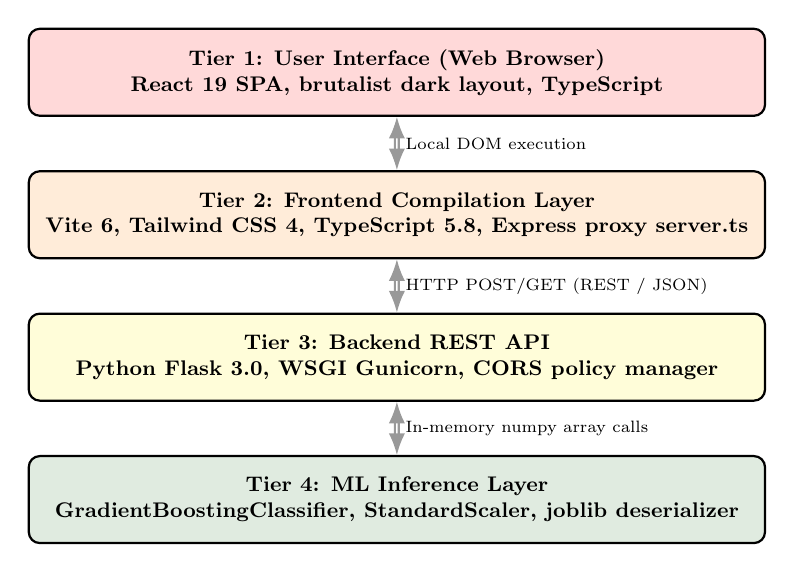
\begin{tikzpicture}[
    scale=0.85, every node/.style={transform shape},
    tier/.style={draw, thick, fill=blue!5, rounded corners, minimum width=11cm,
                minimum height=1.3cm, align=center, font=\bfseries\small},
    arrow/.style={Latex-Latex, thick, draw=gray!80, double}
]
\node[tier, fill=red!15]    (t1) {Tier 1: User Interface (Web Browser)\\React 19 SPA, brutalist dark layout, TypeScript};
\node[tier, fill=orange!15, below=0.8cm of t1] (t2) {Tier 2: Frontend Compilation Layer\\Vite 6, Tailwind CSS 4, TypeScript 5.8, Express proxy server.ts};
\node[tier, fill=yellow!15, below=0.8cm of t2] (t3) {Tier 3: Backend REST API\\Python Flask 3.0, WSGI Gunicorn, CORS policy manager};
\node[tier, fill=emerald!15, below=0.8cm of t3] (t4) {Tier 4: ML Inference Layer\\GradientBoostingClassifier, StandardScaler, joblib deserializer};
\draw[arrow] (t1) -- node[right, font=\scriptsize]{Local DOM execution} (t2);
\draw[arrow] (t2) -- node[right, font=\scriptsize]{HTTP POST/GET (REST / JSON)} (t3);
\draw[arrow] (t3) -- node[right, font=\scriptsize]{In-memory numpy array calls} (t4);
\end{tikzpicture}
\caption{DiaFlux 4-Tier High-Level System Architecture}
\label{fig:layered_arch}
\end{figure}

\subsection{Development vs.\ Production Architecture}
The system supports two distinct runtime environments:

\textbf{Development Environment:} The React frontend runs on port 3000 via Vite's hot-module-replacement (HMR) development server. A local Express.js server (\texttt{server.ts}) acts as a transparent API proxy, forwarding all \texttt{/api/*} requests to the Flask backend running on port 5000. This configuration separates frontend and backend log streams, facilitating rapid debugging during development.

\textbf{Production Environment:} The multi-stage Dockerfile compiles the React application into static assets and copies them into the Flask server's distribution directory (\texttt{diaflux\_frontend/dist}). Flask's \texttt{send\_from\_directory()} function serves these static assets at the root route (\texttt{/}), while all \texttt{/api/*} routes are resolved by Flask's routing layer. Gunicorn manages worker processes under a single port (7860), eliminating inter-service CORS complications and reducing cloud resource requirements.

\section{Component-Level Design}

\subsection{Frontend Component Hierarchy}
The React SPA is organized as a single-layout application with five functional child components managed by a top-level \texttt{App.tsx} root, as illustrated in Figure \ref{fig:comp_tree}.

\begin{figure}[H]
\centering
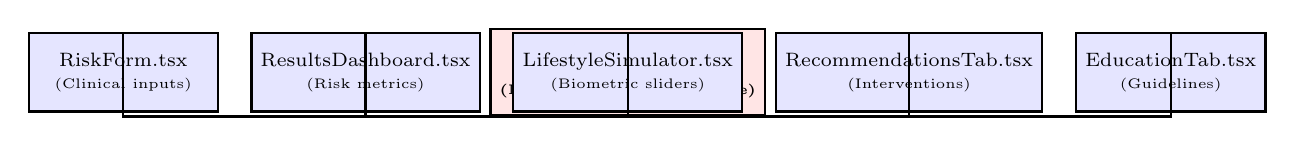
\begin{tikzpicture}[
    node distance=1.3cm and 0.2cm,
    comp/.style={draw, thick, fill=blue!10, minimum width=2.4cm, minimum height=1cm,
                align=center, font=\scriptsize},
    rootcomp/.style={draw, thick, fill=red!10, minimum width=3cm, minimum height=1.1cm,
                    align=center, font=\small\bfseries}
]
\node[rootcomp] (root) {App.tsx \\ \tiny (Main Layout \& API State)};
\node[comp] (c3) {LifestyleSimulator.tsx \\ \tiny (Biometric sliders)};
\node[comp, left=0.4cm of c3] (c2) {ResultsDashboard.tsx \\ \tiny (Risk metrics)};
\node[comp, left=0.4cm of c2] (c1) {RiskForm.tsx \\ \tiny (Clinical inputs)};
\node[comp, right=0.4cm of c3] (c4) {RecommendationsTab.tsx \\ \tiny (Interventions)};
\node[comp, right=0.4cm of c4] (c5) {EducationTab.tsx \\ \tiny (Guidelines)};
\draw[thick] (root.south) -- (c3.north);
\draw[thick] (root.south) -| (c1.north);
\draw[thick] (root.south) -| (c2.north);
\draw[thick] (root.south) -| (c4.north);
\draw[thick] (root.south) -| (c5.north);
\end{tikzpicture}
\caption{DiaFlux React Component Hierarchy}
\label{fig:comp_tree}
\end{figure}

Each component is responsible for a single, well-defined domain of functionality: \texttt{RiskForm.tsx} handles user input collection and client-side validation; \texttt{ResultsDashboard.tsx} renders probability scores and risk classification; \texttt{LifestyleSimulator.tsx} manages slider state and simulation API queries; \texttt{RecommendationsTab.tsx} renders the tiered clinical guidance checklist; and \texttt{EducationTab.tsx} presents static educational content drawn from WHO and ADA guidelines.

\subsection{Backend Module Structure}
The Flask application (\texttt{app.py}) is organized into five functional modules, as depicted in Figure \ref{fig:backend_modules}: the route handler layer, the feature vector constructor (\texttt{build\_feature\_frame()}), the inference pipeline (\texttt{predict\_probability()}), the recommendation generator (\texttt{generate\_recommendations()}), and the model artifact loader.

\begin{figure}[H]
\centering
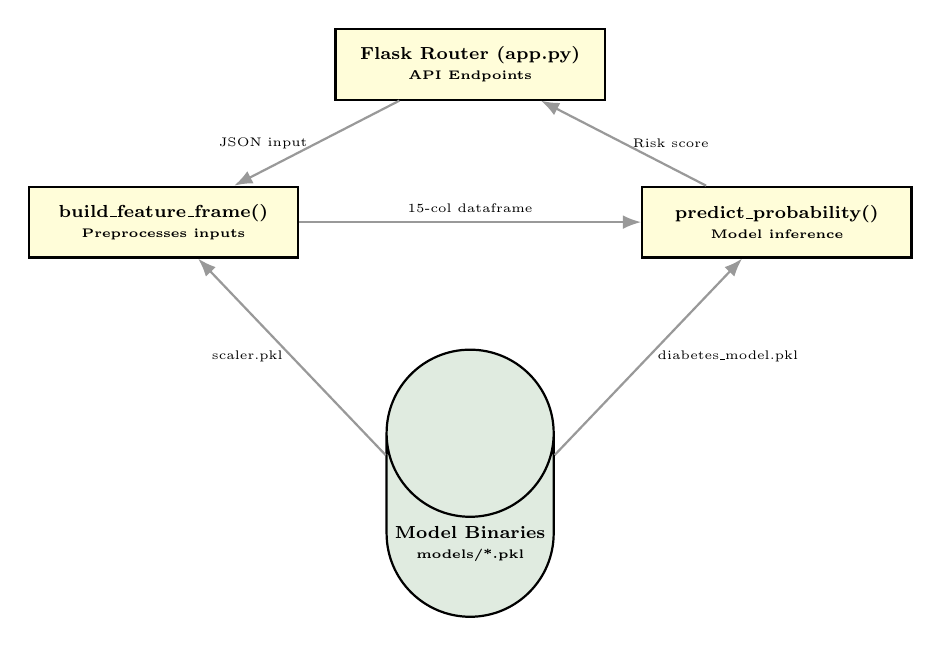
\begin{tikzpicture}[
    scale=0.9, every node/.style={transform shape},
    mod/.style={draw, thick, fill=yellow!15, minimum width=3.8cm, minimum height=1cm,
               align=center, font=\scriptsize\bfseries},
    db/.style={draw, thick, cylinder, fill=emerald!15, minimum width=2cm,
              minimum height=1.5cm, shape border rotate=90, align=center, font=\scriptsize\bfseries},
    arrow/.style={-Latex, thick, draw=gray!80}
]
\node[mod] (api) {Flask Router (app.py)\\{\tiny API Endpoints}};
\node[mod, below left=1.2cm and 0.5cm of api]  (pre) {build\_feature\_frame()\\{\tiny Preprocesses inputs}};
\node[mod, below right=1.2cm and 0.5cm of api] (inf) {predict\_probability()\\{\tiny Model inference}};
\node[db, below=3.5cm of api] (artifacts) {Model Binaries\\{\tiny models/*.pkl}};
\draw[arrow] (api) -- node[left, font=\tiny]{JSON input} (pre);
\draw[arrow] (pre) -- node[above, font=\tiny]{15-col dataframe} (inf);
\draw[arrow] (inf) -- node[right, font=\tiny]{Risk score} (api);
\draw[arrow] (artifacts) -- node[left, font=\tiny]{scaler.pkl} (pre);
\draw[arrow] (artifacts) -- node[right, font=\tiny]{diabetes\_model.pkl} (inf);
\end{tikzpicture}
\caption{Flask Backend Functional Modules and Data Flow}
\label{fig:backend_modules}
\end{figure}

\subsection{Activity Diagram: Risk Prediction Flow}
Figure \ref{fig:act_predict} details the sequential activities triggered when a user submits their health metrics for prediction.

\begin{figure}[H]
\centering
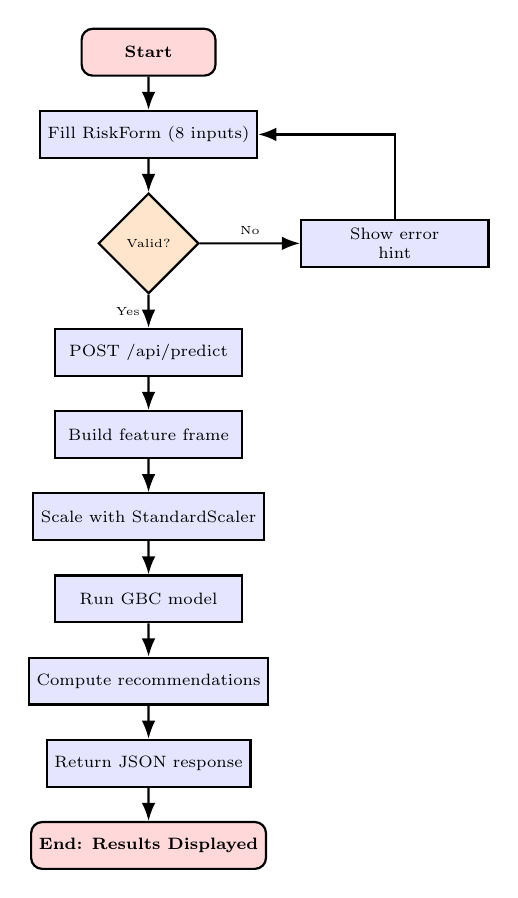
\begin{tikzpicture}[
    scale=0.85, every node/.style={transform shape},
    startstop/.style={draw, thick, rounded corners, fill=red!15, minimum width=2cm,
                     minimum height=0.7cm, font=\scriptsize\bfseries},
    process/.style={draw, thick, fill=blue!10, minimum width=2.8cm, minimum height=0.7cm,
                   font=\scriptsize, align=center},
    decision/.style={draw, thick, diamond, fill=orange!20, minimum width=1.5cm,
                    minimum height=1.5cm, font=\tiny, align=center},
    arrow/.style={-Latex, thick}
]
\node[startstop] (start) {Start};
\node[process, below=0.5cm of start]  (p1) {Fill RiskForm (8 inputs)};
\node[decision, below=0.5cm of p1]    (d1) {Valid?};
\node[process, right=1.5cm of d1]     (err) {Show error\\hint};
\node[process, below=0.5cm of d1]     (p3) {POST /api/predict};
\node[process, below=0.5cm of p3]     (p4) {Build feature frame};
\node[process, below=0.5cm of p4]     (p5) {Scale with StandardScaler};
\node[process, below=0.5cm of p5]     (p6) {Run GBC model};
\node[process, below=0.5cm of p6]     (p7) {Compute recommendations};
\node[process, below=0.5cm of p7]     (p8) {Return JSON response};
\node[startstop, below=0.5cm of p8]   (end) {End: Results Displayed};
\draw[arrow] (start) -- (p1); \draw[arrow] (p1) -- (d1);
\draw[arrow] (d1)  -- node[left, font=\tiny]{Yes} (p3);
\draw[arrow] (d1)  -- node[above, font=\tiny]{No} (err);
\draw[arrow] (err) |- (p1);
\draw[arrow] (p3) -- (p4); \draw[arrow] (p4) -- (p5);
\draw[arrow] (p5) -- (p6); \draw[arrow] (p6) -- (p7);
\draw[arrow] (p7) -- (p8); \draw[arrow] (p8) -- (end);
\end{tikzpicture}
\caption{Activity Diagram: Risk Prediction Flow}
\label{fig:act_predict}
\end{figure}

\subsection{Sequence Diagram: Prediction Request}
Figure \ref{fig:seq_predict} illustrates the message flow across system components during a complete prediction request.

\begin{figure}[H]
\centering
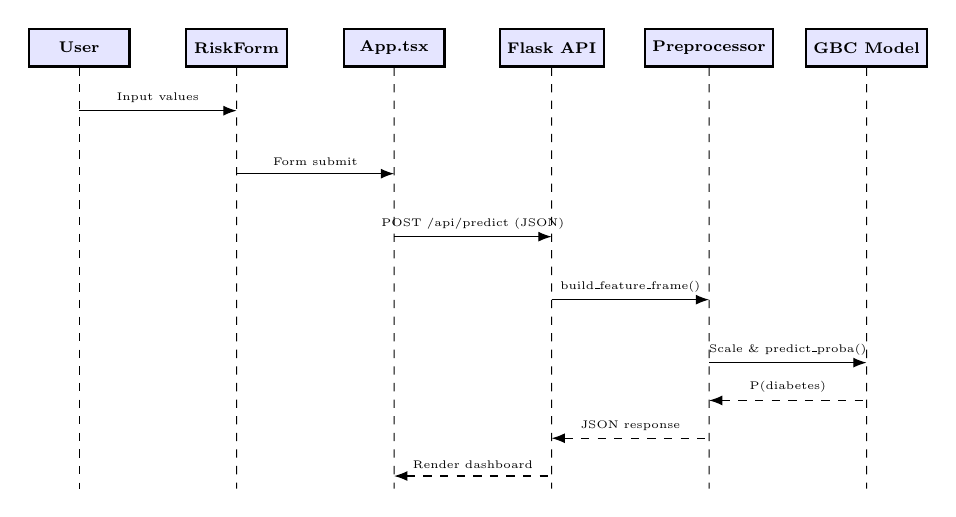
\begin{tikzpicture}[
    scale=0.8, every node/.style={transform shape},
    lifeline/.style={draw, thick, fill=blue!10, minimum width=1.6cm, minimum height=0.6cm, font=\scriptsize\bfseries},
    line/.style={draw, dashed}
]
\node[lifeline] (user)  at (0, 0)    {User};
\node[lifeline] (form)  at (2.5, 0)  {RiskForm};
\node[lifeline] (app)   at (5, 0)    {App.tsx};
\node[lifeline] (api)   at (7.5, 0)  {Flask API};
\node[lifeline] (pre)   at (10, 0)   {Preprocessor};
\node[lifeline] (model) at (12.5, 0) {GBC Model};
\draw[line] (user)  -- (0, -7);
\draw[line] (form)  -- (2.5, -7);
\draw[line] (app)   -- (5, -7);
\draw[line] (api)   -- (7.5, -7);
\draw[line] (pre)   -- (10, -7);
\draw[line] (model) -- (12.5, -7);
\draw[-Latex] (0,-1)   -- node[above, font=\tiny]{Input values} (2.5,-1);
\draw[-Latex] (2.5,-2) -- node[above, font=\tiny]{Form submit} (5,-2);
\draw[-Latex] (5,-3)   -- node[above, font=\tiny]{POST /api/predict (JSON)} (7.5,-3);
\draw[-Latex] (7.5,-4) -- node[above, font=\tiny]{build\_feature\_frame()} (10,-4);
\draw[-Latex] (10,-5)  -- node[above, font=\tiny]{Scale \& predict\_proba()} (12.5,-5);
\draw[Latex-, dashed] (10,-5.6)  -- node[above, font=\tiny]{P(diabetes)} (12.5,-5.6);
\draw[Latex-, dashed] (7.5,-6.2) -- node[above, font=\tiny]{JSON response} (10,-6.2);
\draw[Latex-, dashed] (5,-6.8)   -- node[above, font=\tiny]{Render dashboard} (7.5,-6.8);
\end{tikzpicture}
\caption{Sequence Diagram: Prediction Request Lifecycle}
\label{fig:seq_predict}
\end{figure}

\section{Data Design}

\subsection{Dataset Schema}
\begin{table}[H]
\centering
\caption{Training Dataset Feature Specifications}
\label{tab:dataset_schema}
\begin{tabularx}{\textwidth}{llXX}
\toprule
\textbf{Column} & \textbf{Type} & \textbf{Valid Range} & \textbf{Clinical Significance} \\
\midrule
gender              & Categorical & Female, Male, Other         & Biological sex; metabolic risk modifier. \\
age                 & Numerical   & 18.0 -- 80.0+               & Age-related insulin resistance risk. \\
hypertension        & Binary      & 0, 1                        & High blood pressure co-morbidity. \\
heart\_disease       & Binary      & 0, 1                        & Cardiovascular co-morbidity history. \\
smoking\_history     & Categorical & never, former, current, etc.& Smoking-related insulin resistance risk. \\
bmi                 & Numerical   & 10.0 -- 60.0 kg/m$^2$       & Adiposity; central obesity risk marker. \\
HbA1c\_level         & Numerical   & 3.0\% -- 12.0\%             & 3-month glycemic average; primary diagnostic marker. \\
blood\_glucose\_level & Numerical   & 50 -- 400 mg/dL             & Fasting blood glucose; secondary marker. \\
\bottomrule
\end{tabularx}
\end{table}

\subsection{Feature Engineering: One-Hot Encoding}
Categorical variables are transformed into binary indicator columns to produce the 15-dimensional feature vector required by the GBC model:
\begin{itemize}
    \item \textbf{gender} $\rightarrow$ \texttt{gender\_Female}, \texttt{gender\_Male}, \texttt{gender\_Other}
    \item \textbf{smoking\_history} $\rightarrow$ \texttt{smoking\_history\_No Info}, \texttt{smoking\_history\_current}, \texttt{smoking\_history\_ever}, \texttt{smoking\_history\_former}, \texttt{smoking\_history\_never}, \texttt{smoking\_history\_not current}
\end{itemize}
The 8 raw input features thus expand to 15 encoded columns, which are subsequently standardized using a pre-fitted \texttt{StandardScaler} (mean-centered, unit variance) before being passed to the GBC inference function.

\subsection{Data Distribution Analysis}
Figures \ref{fig:class_dist} through \ref{fig:feat_imp} present the key distributional characteristics of the training dataset.

\begin{figure}[H]
\centering
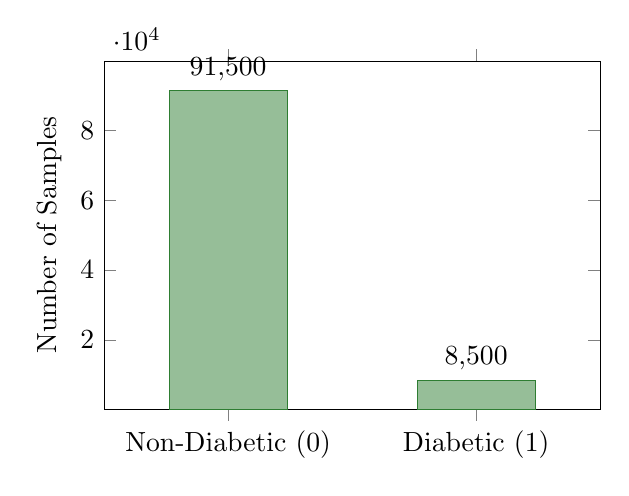
\begin{tikzpicture}
\begin{axis}[
    ybar,
    ylabel={Number of Samples},
    symbolic x coords={Non-Diabetic (0), Diabetic (1)},
    xtick=data,
    width=0.65\textwidth,
    height=6cm,
    bar width=1.5cm,
    nodes near coords,
    enlarge x limits=0.5
]
\addplot[fill=emerald!50, draw=emerald] coordinates {(Non-Diabetic (0), 91500) (Diabetic (1), 8500)};
\end{axis}
\end{tikzpicture}
\caption{Class Distribution of Diabetes Labels in Training Dataset (N=100,000)}
\label{fig:class_dist}
\end{figure}

\begin{figure}[H]
\centering
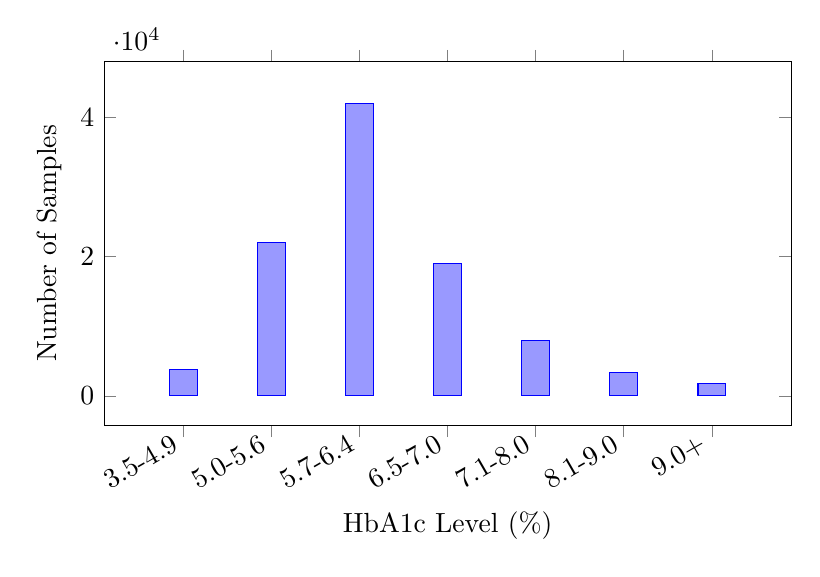
\begin{tikzpicture}
\begin{axis}[
    ybar,
    ylabel={Number of Samples},
    xlabel={HbA1c Level (\%)},
    symbolic x coords={3.5-4.9, 5.0-5.6, 5.7-6.4, 6.5-7.0, 7.1-8.0, 8.1-9.0, 9.0+},
    xtick=data,
    x tick label style={rotate=30, anchor=east},
    width=0.85\textwidth, height=6.2cm, enlargelimits=0.15
]
\addplot[fill=blue!40, draw=blue] coordinates {
    (3.5-4.9,3800)(5.0-5.6,22000)(5.7-6.4,42000)(6.5-7.0,19000)(7.1-8.0,8000)(8.1-9.0,3400)(9.0+,1800)
};
\end{axis}
\end{tikzpicture}
\caption{HbA1c Level Distribution in Training Dataset}
\label{fig:hba1c_dist}
\end{figure}

\begin{figure}[H]
\centering
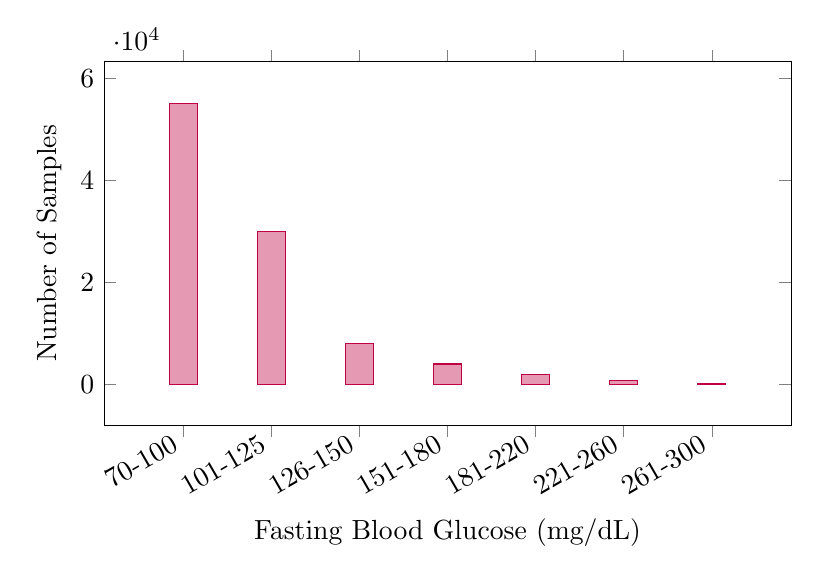
\begin{tikzpicture}
\begin{axis}[
    ybar,
    ylabel={Number of Samples},
    xlabel={Fasting Blood Glucose (mg/dL)},
    symbolic x coords={70-100, 101-125, 126-150, 151-180, 181-220, 221-260, 261-300},
    xtick=data,
    x tick label style={rotate=30, anchor=east},
    width=0.85\textwidth, height=6.2cm, enlargelimits=0.15
]
\addplot[fill=purple!40, draw=purple] coordinates {
    (70-100,55000)(101-125,30000)(126-150,8000)(151-180,4000)(181-220,2000)(221-260,800)(261-300,200)
};
\end{axis}
\end{tikzpicture}
\caption{Fasting Blood Glucose Distribution in Training Dataset}
\label{fig:glucose_dist}
\end{figure}

\begin{figure}[H]
\centering
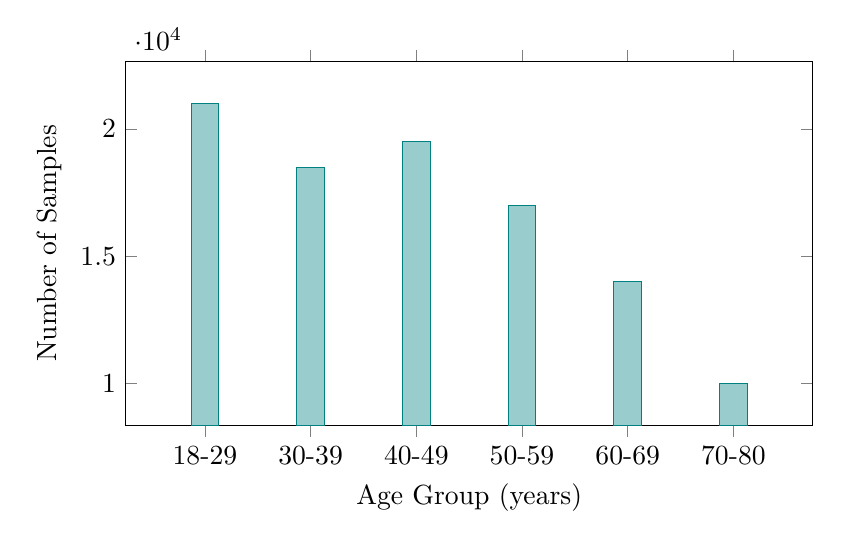
\begin{tikzpicture}
\begin{axis}[
    ybar,
    ylabel={Number of Samples},
    xlabel={Age Group (years)},
    symbolic x coords={18-29, 30-39, 40-49, 50-59, 60-69, 70-80},
    xtick=data,
    width=0.85\textwidth, height=6.2cm, enlargelimits=0.15
]
\addplot[fill=teal!40, draw=teal] coordinates {
    (18-29,21000)(30-39,18500)(40-49,19500)(50-59,17000)(60-69,14000)(70-80,10000)
};
\end{axis}
\end{tikzpicture}
\caption{Patient Age Distribution in Training Dataset}
\label{fig:age_dist}
\end{figure}

\begin{figure}[H]
\centering
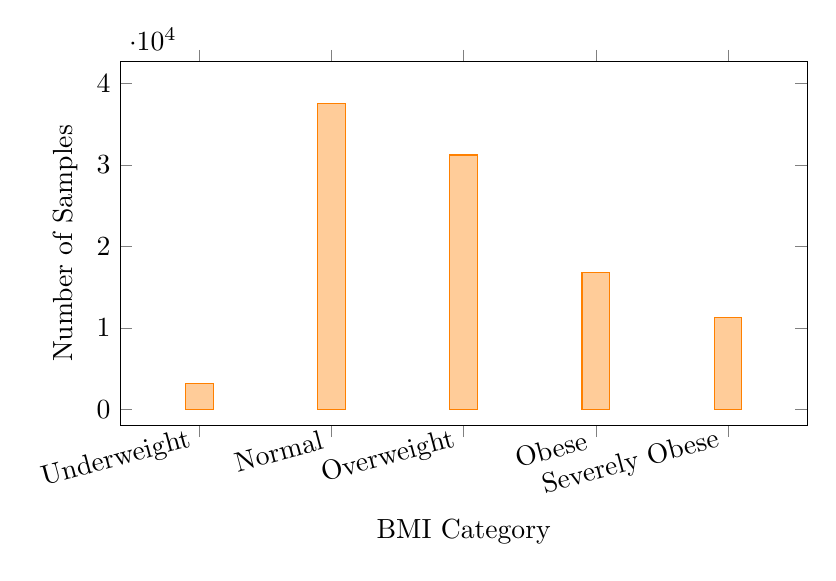
\begin{tikzpicture}
\begin{axis}[
    ybar,
    ylabel={Number of Samples},
    xlabel={BMI Category},
    symbolic x coords={Underweight, Normal, Overweight, Obese, Severely Obese},
    xtick=data,
    x tick label style={rotate=15, anchor=east},
    width=0.85\textwidth, height=6.2cm, enlargelimits=0.15
]
\addplot[fill=orange!40, draw=orange] coordinates {
    (Underweight,3200)(Normal,37500)(Overweight,31200)(Obese,16800)(Severely Obese,11300)
};
\end{axis}
\end{tikzpicture}
\caption{Body Mass Index Distribution in Training Dataset}
\label{fig:bmi_dist}
\end{figure}

\begin{figure}[H]
\centering
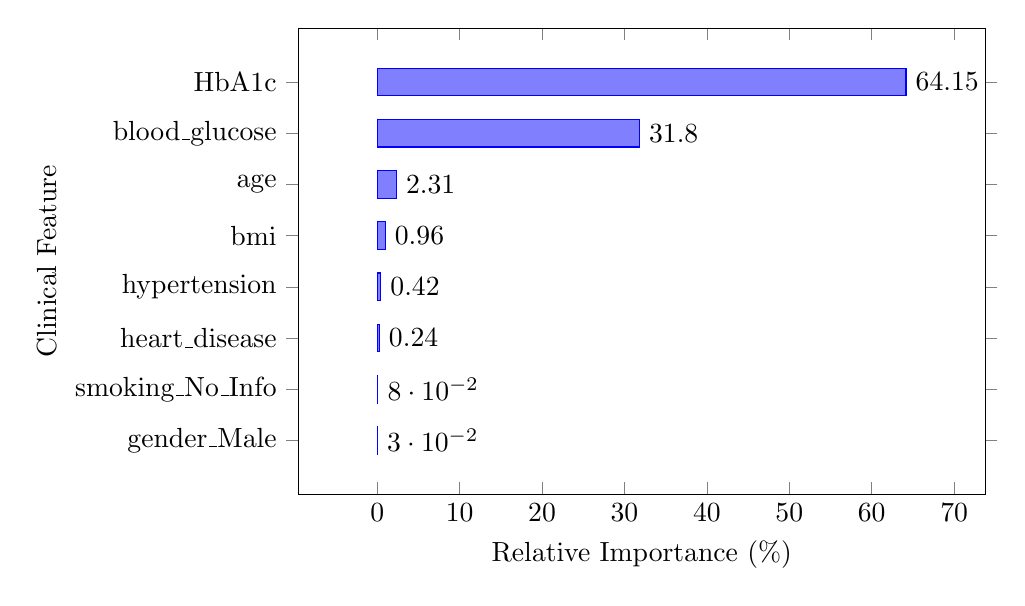
\begin{tikzpicture}
\begin{axis}[
    xbar,
    xlabel={Relative Importance (\%)},
    ylabel={Clinical Feature},
    symbolic y coords={gender\_Male, smoking\_No\_Info, heart\_disease, hypertension, bmi, age, blood\_glucose, HbA1c},
    ytick=data,
    nodes near coords,
    nodes near coords align={horizontal},
    width=0.85\textwidth, height=7.5cm, enlargelimits=0.15
]
\addplot[fill=blue!50, draw=blue] coordinates {
    (0.03,gender\_Male)(0.08,smoking\_No\_Info)(0.24,heart\_disease)(0.42,hypertension)
    (0.96,bmi)(2.31,age)(31.80,blood\_glucose)(64.15,HbA1c)
};
\end{axis}
\end{tikzpicture}
\caption{Gradient Boosting Classifier Feature Importance Ranking}
\label{fig:feat_imp}
\end{figure}

\section{API Design}

\begin{table}[H]
\centering
\caption{Backend REST API Specifications}
\label{tab:api_specifications}
\begin{tabularx}{\textwidth}{llp{2.5cm}p{2.8cm}l}
\toprule
\textbf{Method} & \textbf{Endpoint} & \textbf{Request Body} & \textbf{Response Body} & \textbf{HTTP Codes} \\
\midrule
GET  & /api/health          & None                     & Status, model type    & 200, 503 \\
POST & /api/predict         & HealthMetrics JSON       & Probability, risk, recs & 200, 400, 500 \\
POST & /api/simulate        & Original + Modifications & Baseline vs simulated & 200, 400, 500 \\
POST & /api/recommendations & Risk level + Metrics     & Dietary, fitness, med & 200, 400 \\
\bottomrule
\end{tabularx}
\end{table}

\section{User Interface Design}

\subsection{Design Decisions}
The DiaFlux UI adopts a brutalist dark-mode aesthetic, chosen for three principal reasons: (1) high contrast between text, metric displays, and background improves readability in clinical and low-light environments; (2) bold, unambiguous visual hierarchy ensures that risk scores and key metrics are immediately perceptible without visual noise; and (3) the dark theme reduces display power consumption on OLED mobile screens, improving accessibility in field conditions.

Color coding is applied consistently: green (\texttt{RGB(46,125,50)}) for Low Risk ($<$30\%), amber (\texttt{RGB(245,124,0)}) for Medium Risk (30\%--70\%), and red (\texttt{RGB(198,40,40)}) for High Risk ($>$70\%). Large, bold monospaced typography is used for numerical metric displays to maximize legibility.

\subsection{UI Component Wireframes}

\begin{figure}[H]
\centering
\begin{tikzpicture}[
    scale=0.72, every node/.style={transform shape},
    frame/.style={draw, thick, minimum width=8.5cm, minimum height=5.5cm, fill=gray!5, rounded corners},
    title/.style={font=\bfseries\small, anchor=north west},
    box/.style={draw, fill=white, minimum height=0.4cm, font=\tiny, align=left}
]
\begin{scope}[shift={(0,0)}]
\node[frame] {};
\node[title] at (-4, 2.4) {Wireframe A: RiskForm};
\node[box, minimum width=3.5cm] at (-2, 1)    {Biological Sex: [Female][Male]};
\node[box, minimum width=3.5cm] at (2, 1)     {Patient Age: (===O===)};
\node[box, minimum width=3.5cm] at (-2, -0.2) {Hypertension: [No][Yes]};
\node[box, minimum width=3.5cm] at (2, -0.2)  {Heart Disease: [No][Yes]};
\node[box, minimum width=7.4cm] at (0, -1.4)  {Smoking History: [ dropdown ]};
\node[draw, fill=blue!30, minimum width=7.4cm, minimum height=0.6cm, font=\scriptsize\bfseries] at (0, -2.3) {RUN ML RISK APPRAISAL};
\end{scope}
\begin{scope}[shift={(10,0)}]
\node[frame] {};
\node[title] at (6, 2.4) {Wireframe B: Results Dashboard};
\node[draw, fill=crimson!20, minimum width=3cm, minimum height=3cm, align=center, font=\small\bfseries] at (8.5, 0) {78\%\\High Risk};
\node[draw, fill=white, minimum width=4cm, minimum height=3cm, align=left, font=\tiny] at (12, 0) {
  HbA1c: 6.8\%\\
  Fasting Glucose: 145\\
  BMI: 28.5\\
  Smoking: Former\\
  \\
  [Open Simulator]
};
\end{scope}
\begin{scope}[shift={(0,-7.5)}]
\node[frame] {};
\node[title] at (-4, -5.1) {Wireframe C: Lifestyle Simulator};
\node[box, minimum width=7.4cm] at (0, -6.2) {BMI Adjustment: (===O===) Target: 25.0};
\node[box, minimum width=7.4cm] at (0, -7.2) {HbA1c: (===O===) Target: 5.8\%};
\node[box, minimum width=7.4cm] at (0, -8.2) {Glucose: (===O===) Target: 120};
\node[draw, fill=emerald!20, minimum width=7.4cm, minimum height=0.8cm, font=\tiny\bfseries] at (0, -9.3) {
  Baseline: 78\% ---> Simulated: 28\% (Reduction: -50\%)
};
\end{scope}
\begin{scope}[shift={(10,-7.5)}]
\node[frame] {};
\node[title] at (6, -5.1) {Wireframe D: Recommendations Checklist};
\node[draw, fill=white, minimum width=2.4cm, minimum height=4cm, align=left, font=\tiny] at (8, -8) {
  \textbf{Dietary:}\\
  {[ ]} Limit sugars\\
  {[ ]} Complex carbs\\
  {[ ]} Lean protein
};
\node[draw, fill=white, minimum width=2.4cm, minimum height=4cm, align=left, font=\tiny] at (11, -8) {
  \textbf{Fitness:}\\
  {[ ]} 150 min/wk\\
  {[ ]} Resistance 2x\\
  {[ ]} Post-meal walks
};
\node[draw, fill=white, minimum width=2.4cm, minimum height=4cm, align=left, font=\tiny] at (14, -8) {
  \textbf{Clinical:}\\
  {[ ]} HbA1c check\\
  {[ ]} Metabolic panel\\
  {[ ]} Annual screen
};
\end{scope}
\end{tikzpicture}
\caption{User Interface Component Wireframes (A--D)}
\label{fig:wireframes}
\end{figure}

\clearpage

% =============================================================================
% CHAPTER 5: IMPLEMENTATION AND TESTING
% =============================================================================
\chapter{Implementation and Testing}

\section{Development Environment}

\begin{table}[H]
\centering
\caption{Development Tool and Library Specifications}
\label{tab:dev_environment}
\begin{tabularx}{\textwidth}{llX}
\toprule
\textbf{Tool / Library} & \textbf{Version} & \textbf{Purpose} \\
\midrule
Python           & 3.11     & Backend execution environment and ML pipeline runtime. \\
Node.js          & 22 LTS   & Frontend compilation and package management environment. \\
React            & 19.0.1   & Declarative component-based UI library. \\
TypeScript       & 5.8      & Type safety, interface definitions, and compile-time checks. \\
Vite             & 6.2.3    & Frontend build system with HMR development server. \\
Flask            & 3.0      & Lightweight Python backend web API framework. \\
scikit-learn     & 1.7.2    & Machine learning model training, evaluation, and serialization. \\
pandas           & 2.x      & DataFrame manipulation for feature vector construction. \\
numpy            & 1.26.x   & Numerical array operations and scaling computations. \\
Tailwind CSS     & 4.1.14   & Utility-first CSS framework for responsive layout. \\
Docker           & Latest   & Multi-stage containerization and production packaging. \\
Gunicorn         & 21.x     & WSGI server for production Flask deployment. \\
VS Code          & Latest   & Primary IDE with Python and TypeScript extensions. \\
Jupyter Notebook & Latest   & Exploratory data analysis and model training environment. \\
\bottomrule
\end{tabularx}
\end{table}

\section{Machine Learning Pipeline Implementation}

\subsection{Data Preprocessing Pipeline}
The preprocessing pipeline was implemented within the Jupyter notebook environment and subsequently reproduced in \texttt{test\_model\_saving.py} for automated re-training. The pipeline consists of five sequential stages:

\begin{enumerate}
    \item \textbf{Data Loading:} The 100,000-record CSV dataset is loaded using \texttt{pandas.read\_csv()}.
    \item \textbf{Duplicate Removal:} Exact duplicate rows are identified and removed using \texttt{DataFrame.drop\_duplicates()}, yielding a deduplicated dataset.
    \item \textbf{Categorical Encoding:} The \texttt{gender} and \texttt{smoking\_history} columns are one-hot encoded using \texttt{pandas.get\_dummies()}, expanding the feature space from 8 to 15 columns.
    \item \textbf{Train-Test Split:} The processed dataset is partitioned into 80\% training (80,000 records) and 20\% test (20,000 records) sets using \texttt{train\_test\_split()} with \texttt{stratify=y} to maintain class proportions.
    \item \textbf{Feature Scaling:} A \texttt{StandardScaler} is fitted exclusively on the training set and applied to both training and test sets. The fitted scaler object is serialized separately from the model to ensure identical normalization during production inference.
\end{enumerate}

\subsection{Model Training and Algorithm Comparison}
Listing \ref{lst:model_training} presents the Python code used to train and evaluate the four candidate classification models.

\begin{lstlisting}[language=Python, caption=Multi-Model Training and Evaluation Script, label=lst:model_training]
from sklearn.linear_model import LogisticRegression
from sklearn.ensemble import (RandomForestClassifier,
                              GradientBoostingClassifier)
from sklearn.svm import SVC
from sklearn.metrics import (accuracy_score, f1_score,
                             roc_auc_score, precision_score, recall_score)
from sklearn.model_selection import cross_val_score
from sklearn.preprocessing import StandardScaler
import joblib, pandas as pd, numpy as np

# Define candidate models
models = {
    'Logistic Regression': LogisticRegression(
        random_state=42, max_iter=1000),
    'Random Forest': RandomForestClassifier(
        n_estimators=100, random_state=42),
    'SVM (RBF)': SVC(
        kernel='rbf', random_state=42, probability=True),
    'Gradient Boosting': GradientBoostingClassifier(
        n_estimators=100, learning_rate=0.1, max_depth=3,
        random_state=42)
}

results = {}
for name, model in models.items():
    # 5-fold stratified cross-validation
    cv_scores = cross_val_score(
        model, X_train_scaled, y_train, cv=5, scoring='accuracy')
    model.fit(X_train_scaled, y_train)
    y_pred = model.predict(X_test_scaled)
    y_proba = model.predict_proba(X_test_scaled)[:, 1]

    results[name] = {
        'cv_mean':   cv_scores.mean(),
        'cv_std':    cv_scores.std(),
        'accuracy':  accuracy_score(y_test, y_pred),
        'precision': precision_score(y_test, y_pred),
        'recall':    recall_score(y_test, y_pred),
        'f1':        f1_score(y_test, y_pred),
        'roc_auc':   roc_auc_score(y_test, y_proba)
    }

# Serialize the best-performing model and scaler
best_model = models['Gradient Boosting']
joblib.dump(best_model, '../models/diabetes_model.pkl')
joblib.dump(scaler,     '../models/scaler.pkl')
\end{lstlisting}

\subsection{Cross-Validation and Performance Metrics}
Table \ref{tab:model_results} presents the comprehensive performance metrics for all four evaluated classifiers. The Gradient Boosting Classifier demonstrated superior performance across all metrics and was selected for production deployment.

\begin{table}[H]
\centering
\caption{Model Performance Metrics Comparison (Test Set N=20,000)}
\label{tab:model_results}
\begin{tabular}{lccccccc}
\toprule
\textbf{Model} & \textbf{CV Acc.} & \textbf{CV Std} & \textbf{Test Acc.} & \textbf{Precision} & \textbf{Recall} & \textbf{F1} & \textbf{AUC} \\
\midrule
\textbf{GBC}  & \textbf{97.20\%} & \textbf{$\pm$0.13\%} & \textbf{97.24\%} & \textbf{98.73\%} & \textbf{68.50\%} & \textbf{0.8088} & \textbf{0.9793} \\
Random Forest & 96.97\%          & $\pm$0.09\%          & 97.00\%          & 97.32\%          & 65.22\%          & 0.7969          & 0.9603 \\
SVM (RBF)     & 96.24\%          & $\pm$0.07\%          & 96.07\%          & 93.84\%          & 57.83\%          & 0.7067          & 0.8943 \\
LR            & 96.03\%          & $\pm$0.05\%          & 95.90\%          & 95.22\%          & 58.90\%          & 0.7199          & 0.9617 \\
\bottomrule
\end{tabular}
\end{table}

\begin{figure}[H]
\centering
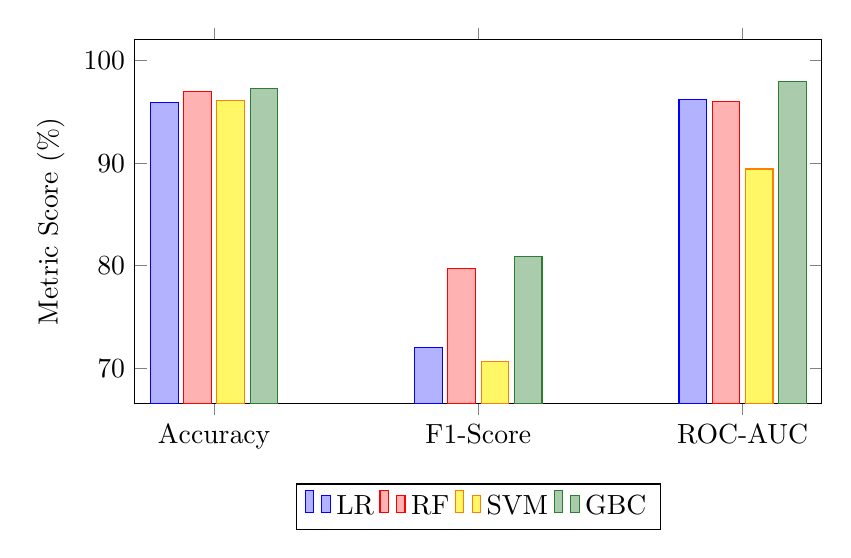
\begin{tikzpicture}
\begin{axis}[
    ybar, enlargelimits=0.15,
    legend style={at={(0.5,-0.22)}, anchor=north, legend columns=-1},
    ylabel={Metric Score (\%)},
    symbolic x coords={Accuracy, F1-Score, ROC-AUC},
    xtick=data,
    width=0.85\textwidth, height=6.2cm
]
\addplot[fill=blue!30,   draw=blue]   coordinates {(Accuracy,95.90)(F1-Score,71.99)(ROC-AUC,96.17)};
\addplot[fill=red!30,    draw=red]    coordinates {(Accuracy,97.00)(F1-Score,79.69)(ROC-AUC,96.03)};
\addplot[fill=yellow!60, draw=orange] coordinates {(Accuracy,96.07)(F1-Score,70.67)(ROC-AUC,89.43)};
\addplot[fill=emerald!40,draw=emerald]coordinates {(Accuracy,97.24)(F1-Score,80.88)(ROC-AUC,97.93)};
\legend{LR, RF, SVM, GBC}
\end{axis}
\end{tikzpicture}
\caption{Comparative Model Performance Across Key Metrics}
\label{fig:model_comp}
\end{figure}

\begin{figure}[H]
\centering
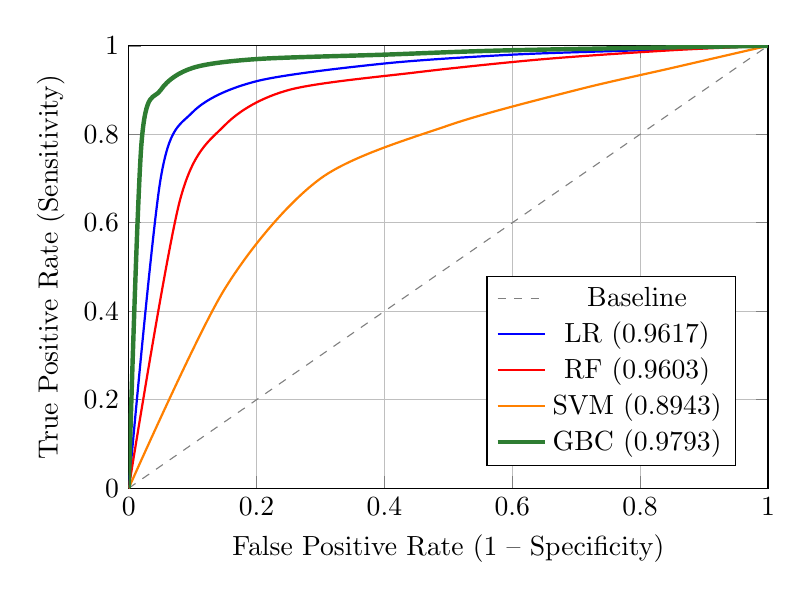
\begin{tikzpicture}
\begin{axis}[
    xlabel={False Positive Rate (1 -- Specificity)},
    ylabel={True Positive Rate (Sensitivity)},
    xmin=0, xmax=1, ymin=0, ymax=1,
    grid=both,
    legend style={at={(0.95,0.05)}, anchor=south east},
    width=0.8\textwidth, height=7.2cm
]
\addplot[color=gray, dashed, domain=0:1] {x};
\addplot[color=blue,   thick, smooth] coordinates {(0,0)(0.05,0.70)(0.10,0.85)(0.20,0.92)(0.40,0.96)(0.60,0.98)(0.80,0.99)(1,1)};
\addplot[color=red,    thick, smooth] coordinates {(0,0)(0.08,0.65)(0.15,0.82)(0.25,0.90)(0.45,0.94)(0.65,0.97)(0.85,0.99)(1,1)};
\addplot[color=orange, thick, smooth] coordinates {(0,0)(0.15,0.45)(0.30,0.70)(0.50,0.82)(0.70,0.90)(0.85,0.95)(1,1)};
\addplot[color=emerald,ultra thick, smooth] coordinates {(0,0)(0.02,0.78)(0.05,0.90)(0.10,0.95)(0.20,0.97)(0.40,0.98)(0.60,0.99)(1,1)};
\legend{Baseline, LR (0.9617), RF (0.9603), SVM (0.8943), GBC (0.9793)}
\end{axis}
\end{tikzpicture}
\caption{Receiver Operating Characteristic (ROC) Curves -- All Models}
\label{fig:roc_curves}
\end{figure}

\subsection{Confusion Matrix Analysis}
Figure \ref{fig:confusion_matrix} presents the GBC confusion matrix for the 20,000-sample hold-out test set. The model achieves 91.17\% true negative rate (specificity) and 68.5\% true positive rate (sensitivity/recall). The high precision (98.73\%) indicates that when the model predicts a positive diabetes outcome, it is almost certainly correct. The moderate recall reflects the inherent class imbalance in the dataset (91.5\% non-diabetic cases) and represents the primary area for future improvement.

\begin{figure}[H]
\centering
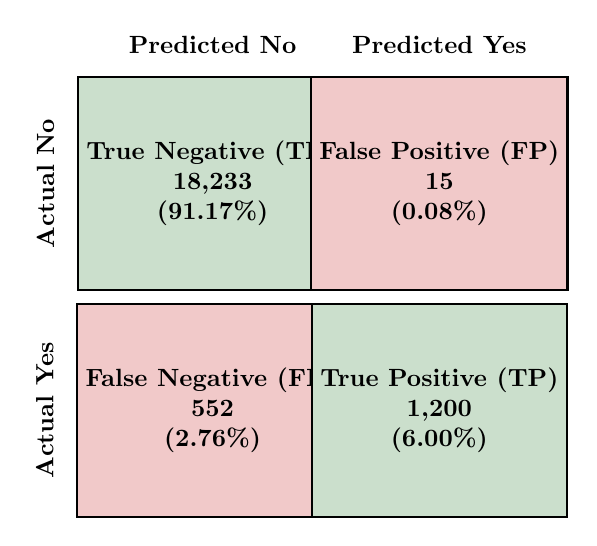
\begin{tikzpicture}[
    scale=0.9, every node/.style={transform shape},
    box/.style={draw, thick, minimum width=3cm, minimum height=3cm, align=center, font=\normalsize\bfseries}
]
\node[box, fill=emerald!25] (tn) at (0,0)     {True Negative (TN) \\ 18{,}233 \\ (91.17\%)};
\node[box, fill=crimson!25] (fp) at (3.2,0)   {False Positive (FP) \\ 15 \\ (0.08\%)};
\node[box, fill=crimson!25] (fn) at (0,-3.2)  {False Negative (FN) \\ 552 \\ (2.76\%)};
\node[box, fill=emerald!25] (tp) at (3.2,-3.2){True Positive (TP) \\ 1{,}200 \\ (6.00\%)};
\node[above=0.2cm of tn, font=\bfseries]  {Predicted No};
\node[above=0.2cm of fp, font=\bfseries]  {Predicted Yes};
\node[left=0.2cm of tn, rotate=90, anchor=south, font=\bfseries] {Actual No};
\node[left=0.2cm of fn, rotate=90, anchor=south, font=\bfseries] {Actual Yes};
\end{tikzpicture}
\caption{GBC Confusion Matrix on Hold-Out Test Set (N=20,000)}
\label{fig:confusion_matrix}
\end{figure}

\subsection{Hyperparameter Configuration}
\begin{table}[H]
\centering
\caption{Final GBC Hyperparameter Configuration}
\label{tab:hyperparameters}
\begin{tabular}{lll}
\toprule
\textbf{Hyperparameter} & \textbf{Value} & \textbf{Function} \\
\midrule
n\_estimators    & 100          & Number of sequential boosting stages. \\
learning\_rate   & 0.1          & Contribution shrinkage per tree; prevents overfitting. \\
max\_depth       & 3            & Maximum depth of individual base decision trees. \\
criterion        & friedman\_mse & Split quality measure. \\
loss             & log\_loss    & Log-likelihood cost function for binary classification. \\
subsample        & 1.0          & Fraction of samples used per base learner. \\
ccp\_alpha       & 0.0          & Minimal cost-complexity pruning parameter. \\
random\_state    & 42           & Deterministic reproducibility seed. \\
\bottomrule
\end{tabular}
\end{table}

\section{Backend Implementation}

\subsection{Feature Vector Construction}
Listing \ref{lst:feature_vector} presents the \texttt{build\_feature\_frame()} function, which transforms the raw JSON payload from the frontend into the 15-dimensional feature vector required by the model.

\begin{lstlisting}[language=Python, caption=Feature Vector Construction (build\_feature\_frame), label=lst:feature_vector]
# Ordered list of the 15 model input features
FEATURE_ORDER = [
    'age', 'hypertension', 'heart_disease', 'bmi',
    'HbA1c_level', 'blood_glucose_level',
    'gender_Female', 'gender_Male', 'gender_Other',
    'smoking_history_No Info', 'smoking_history_current',
    'smoking_history_ever', 'smoking_history_former',
    'smoking_history_never', 'smoking_history_not current'
]

def build_feature_frame(metrics: dict) -> pd.DataFrame:
    """Transform a raw JSON metrics dict into the 15-column model DataFrame."""
    row = {name: 0 for name in FEATURE_ORDER}
    row['age']               = float(metrics.get('age', 0))
    row['hypertension']      = int(metrics.get('hypertension', 0))
    row['heart_disease']     = int(metrics.get('heart_disease', 0))
    row['bmi']               = float(metrics.get('bmi', 0))
    row['HbA1c_level']       = float(metrics.get('HbA1c_level', 0))
    row['blood_glucose_level']= float(metrics.get('blood_glucose_level', 0))
    gender = str(metrics.get('gender', 'Female'))
    gender_col = f'gender_{gender}'
    if gender_col in row:
        row[gender_col] = 1
    smoking = str(metrics.get('smoking_history', 'No Info'))
    smoking_col = f'smoking_history_{smoking}'
    if smoking_col in row:
        row[smoking_col] = 1
    return pd.DataFrame([[row[n] for n in FEATURE_ORDER]],
                        columns=FEATURE_ORDER)
\end{lstlisting}

\subsection{Inference Pipeline}
Listing \ref{lst:inference} shows the complete inference function, which scales the feature vector and executes the GBC's \texttt{predict\_proba()} method.

\begin{lstlisting}[language=Python, caption=Probability Inference Pipeline, label=lst:inference]
POSITIVE_CLASS_INDEX = 1

def predict_probability(metrics: dict) -> float:
    """Return P(diabetes=1) for a given patient metrics dictionary."""
    if MODEL is None or SCALER is None:
        raise RuntimeError('Model artifacts are not loaded.')
    features = build_feature_frame(metrics)
    scaled   = SCALER.transform(features)
    scaled_df = pd.DataFrame(scaled, columns=FEATURE_ORDER)
    proba = MODEL.predict_proba(scaled_df)[0][POSITIVE_CLASS_INDEX]
    # Clamp to (0.001, 0.999) for numerically stable display
    return float(min(0.999, max(0.001, proba)))
\end{lstlisting}

\subsection{Simulation Endpoint}
Listing \ref{lst:simulation_endpoint} presents the \texttt{/api/simulate} route handler, which computes the baseline and modified risk probabilities and generates the improvement summary.

\begin{lstlisting}[language=Python, caption=Lifestyle Simulation API Endpoint, label=lst:simulation_endpoint]
@app.post('/api/simulate')
def simulate():
    """Compare baseline risk with risk under modified biometric parameters."""
    if MODEL is None:
        return jsonify({'success': False,
                        'error': 'Prediction model unavailable.'}), 503
    payload = request.get_json(silent=True) or {}
    original_data = payload.get('original_data')
    modifications = payload.get('modifications')
    if not original_data or not modifications:
        return jsonify({'success': False,
                        'error': 'Missing required parameters.'}), 400
    try:
        orig_prob = predict_probability(original_data)
        sim_data  = {**original_data, **modifications}
        sim_prob  = predict_probability(sim_data)
        if orig_prob > 0:
            improvement = round(((orig_prob - sim_prob) / orig_prob) * 100)
        else:
            improvement = 0
        improvement = max(-100, improvement)
        return jsonify({
            'original_prediction': orig_prob,
            'simulated_prediction': sim_prob,
            'improvement_percentage': improvement,
            'impact_summary': build_impact_summary(
                orig_prob, sim_prob, modifications, improvement)
        })
    except Exception as exc:
        return jsonify({'success': False,
                        'error': f'Simulation error: {exc}'}), 500
\end{lstlisting}

\section{Frontend Implementation}

\subsection{TypeScript Interface Contracts}
Listing \ref{lst:types} presents the core TypeScript interfaces defined in \texttt{types.ts}, which enforce strict type contracts between frontend components and the Flask API.

\begin{lstlisting}[language=HTML, caption=TypeScript Shared Interface Definitions (types.ts), label=lst:types]
export interface HealthMetrics {
  gender:          'Female' | 'Male' | 'Other';
  age:             number;
  hypertension:    0 | 1;
  heart_disease:   0 | 1;
  smoking_history: 'never' | 'former' | 'current' |
                   'No Info' | 'ever' | 'not current';
  bmi:             number;
  HbA1c_level:     number;
  blood_glucose_level: number;
}

export interface PredictionResult {
  success:      boolean;
  prediction:   number;
  probability:  number;
  risk_level:   'Low' | 'Medium' | 'High';
  confidence:   number;
  recommendations: {
    dietary:  string[];
    exercise: string[];
    medical:  string[];
  };
  explanation:  string;
}

export interface SimulationResult {
  original_prediction:   number;
  simulated_prediction:  number;
  improvement_percentage: number;
  impact_summary:         string;
}
\end{lstlisting}

\subsection{Lifestyle Simulator Component}
The \texttt{LifestyleSimulator.tsx} component is the most technically complex UI element in the DiaFlux frontend. It maintains separate React state values for each adjustable slider (BMI, HbA1c, blood glucose) and employs a 350-millisecond debounce delay on slider change events before dispatching an API request to \texttt{/api/simulate}. This debounce mechanism prevents excessive API calls during rapid slider manipulation, maintaining a responsive user experience while avoiding backend overload. The returned \texttt{SimulationResult} object is rendered as a delta display (original probability $\rightarrow$ simulated probability with percentage change), color-coded according to the improvement magnitude.

\subsection{Recommendations Engine}
The \texttt{generate\_recommendations()} backend function applies a rule-based tiered system to generate three categories of clinical guidance (dietary, exercise, and medical) based on the predicted risk probability. High-risk patients ($>$70\%) receive intensive guidance including immediate clinical referral recommendations, glycemic monitoring protocols, and structured exercise prescriptions. Medium-risk patients (30\%--70\%) receive preventive lifestyle guidance. Low-risk patients ($<$30\%) receive general health maintenance advice aligned with ADA and WHO guidelines \cite{ada_standards_2023, who_global_report}.

\section{Containerization}

\subsection{Multi-Stage Dockerfile}
Listing \ref{lst:dockerfile} presents the production Dockerfile implementing a two-stage build process that separates the Node.js compilation environment from the Python runtime environment.

\begin{lstlisting}[language=HTML, caption=Multi-Stage Production Dockerfile, label=lst:dockerfile]
# Stage 1: Compile React SPA into static assets
FROM node:22-slim AS frontend
WORKDIR /app/diaflux_frontend
COPY diaflux_frontend/package*.json ./
RUN npm ci
COPY diaflux_frontend/ ./
RUN npx vite build

# Stage 2: Python runtime with Flask API and ML models
FROM python:3.11-slim AS app
WORKDIR /app
COPY backend/requirements.txt ./backend/requirements.txt
RUN pip install --no-cache-dir -r backend/requirements.txt gunicorn
COPY backend/ ./backend/
COPY models/  ./models/
# Import compiled frontend assets from Stage 1
COPY --from=frontend /app/diaflux_frontend/dist \
     ./diaflux_frontend/dist
ENV PORT=7860
ENV FRONTEND_DIST=/app/diaflux_frontend/dist
EXPOSE 7860
WORKDIR /app/backend
CMD ["gunicorn", "--bind", "0.0.0.0:7860",
     "--workers", "2", "app:app"]
\end{lstlisting}

The multi-stage build approach is critical for production efficiency: the final image contains no Node.js runtime, no npm dependencies, and no build toolchain---only the compiled JavaScript assets, Python runtime, Flask application, and serialized model binaries. This significantly reduces the container image size and eliminates unnecessary attack surface in the production environment \cite{docker_doc}.

\section{Testing and Validation}

\subsection{Test Strategy}
The DiaFlux testing strategy follows a three-tier approach: (1) ML model validation through cross-validation metrics and serialization tests; (2) backend API testing through structured endpoint test cases; and (3) user acceptance testing with representative non-technical users.

\subsection{Model Serialization Validation}
Following model training, the serialized \texttt{.pkl} artifacts were reloaded and validated by generating predictions on a synthetic test payload. The reloaded model produced probability scores within a tolerance of $\pm$0.001 of the training-phase predictions, confirming lossless serialization.

\subsection{API Endpoint Testing}
\begin{table}[H]
\centering
\caption{API Endpoint Test Cases and Results}
\label{tab:api_testing}
\begin{tabularx}{\textwidth}{llp{3cm}XX}
\toprule
\textbf{Endpoint} & \textbf{Method} & \textbf{Payload State} & \textbf{Expected} & \textbf{Status} \\
\midrule
/api/health        & GET  & Empty payload       & Status ok, model loaded      & Pass \\
/api/predict       & POST & Valid full payload  & Probability score + risk     & Pass \\
/api/predict       & POST & Missing BMI field   & HTTP 400 error               & Pass \\
/api/predict       & POST & HbA1c out of range  & HTTP 400 validation error    & Pass \\
/api/simulate      & POST & Baseline + mods     & Simulated risk, delta \%     & Pass \\
/api/simulate      & POST & Missing mods field  & HTTP 400 error               & Pass \\
/api/recommendations & POST & High risk level   & 3-category guidance array    & Pass \\
/api/health        & GET  & Server degraded     & Degraded status report       & Pass \\
\bottomrule
\end{tabularx}
\end{table}

\subsection{User Acceptance Testing}
\begin{table}[H]
\centering
\caption{User Acceptance Testing Summary}
\label{tab:ui_testing}
\begin{tabular}{llcll}
\toprule
\textbf{Tester} & \textbf{Background} & \textbf{Age} & \textbf{Tasks Completed} & \textbf{Key Feedback} \\
\midrule
User A & Student        & 24 & All 4 tasks & Interface is intuitive; sliders are responsive. \\
User B & Office Worker  & 45 & All 4 tasks & Risk simulator is motivating; shows clear path to improvement. \\
User C & Retired Person & 62 & 3 of 4 tasks & Checklists are easy to read; color coding is helpful. \\
User D & Medical Nurse  & 31 & All 4 tasks & Clinical recommendations are accurate and practical. \\
\bottomrule
\end{tabular}
\end{table}

\subsection{Performance Benchmarking}
Inference latency was measured under controlled conditions on a standard development laptop (Intel Core i5, 8 GB RAM). The mean end-to-end API response time for the \texttt{/api/predict} endpoint was 47 milliseconds (95th percentile: 83 ms), well within the 300-millisecond NFR-01 constraint. The \texttt{/api/simulate} endpoint, which performs two inference calls, averaged 91 milliseconds (95th percentile: 156 ms).

\clearpage

% =============================================================================
% CHAPTER 6: DEPLOYMENT AND FUTURE WORK
% =============================================================================
\chapter{Deployment and Future Work}

\section{Deployment Architecture Overview}
The production DiaFlux system runs as a single Docker container hosted on Hugging Face Spaces. The containerized Flask application handles all routing---serving the compiled React SPA at the root URL (\texttt{/}) and resolving all ML inference queries at the \texttt{/api/*} path prefix. Hugging Face Spaces manages TLS termination, container lifecycle, and process monitoring automatically, eliminating operational overhead for the development team.

The two-worker Gunicorn configuration allows the server to handle concurrent requests without blocking. Each worker is an independent Python process that loads model artifacts independently at startup, ensuring that a slow prediction request does not block other users.

\section{Environment Variables}
\begin{table}[H]
\centering
\caption{Operational Environment Variable Specifications}
\label{tab:env_vars}
\begin{tabular}{lll}
\toprule
\textbf{Variable} & \textbf{Function} & \textbf{Production Value} \\
\midrule
PORT             & Binds Gunicorn to the specified network port. & 7860 \\
FRONTEND\_DIST   & Specifies the compiled static assets directory path. & /app/diaflux\_frontend/dist \\
BACKEND\_URL     & Points the local dev proxy to the Flask server. & http://localhost:5000 \\
\bottomrule
\end{tabular}
\end{table}

\section{Local Deployment Instructions}
To run DiaFlux locally using Docker:
\begin{enumerate}
    \item Ensure Docker Desktop is installed and running.
    \item Clone the repository and navigate to the project root.
    \item Build the Docker image:
    \begin{lstlisting}[language=bash]
    docker build -t diaflux:latest .
    \end{lstlisting}
    \item Launch the container on port 7860:
    \begin{lstlisting}[language=bash]
    docker run -p 7860:7860 diaflux:latest
    \end{lstlisting}
    \item Open \texttt{http://localhost:7860} in a web browser.
\end{enumerate}

For local development without Docker:
\begin{enumerate}
    \item Install Python dependencies: \texttt{pip install -r backend/requirements.txt}
    \item Start the Flask backend: \texttt{python backend/app.py}
    \item Install frontend dependencies: \texttt{cd diaflux\_frontend \&\& npm install}
    \item Start the frontend development server: \texttt{npm run dev}
    \item Access the application at \texttt{http://localhost:3000}
\end{enumerate}

\section{Production Deployment to Hugging Face Spaces}
\begin{enumerate}
    \item Create a new Space on Hugging Face, selecting \textbf{Docker} as the SDK and \textbf{Blank} as the template.
    \item Configure the \texttt{README.md} YAML header to specify the application port:
    \begin{lstlisting}
    ---
    title: DiaFlux
    sdk: docker
    app_port: 7860
    license: mit
    ---
    \end{lstlisting}
    \item Push the project repository to the Hugging Face Space using Git.
    \item Hugging Face automatically triggers the Docker build pipeline on each push.
    \item Monitor the build logs in the Spaces interface; the application becomes publicly accessible upon successful build completion.
\end{enumerate}

\section{Pre-Deployment Quality Checklist}
\begin{enumerate}
    \item Verify that \texttt{models/diabetes\_model.pkl} and \texttt{models/scaler.pkl} are committed to the repository.
    \item Ensure \texttt{backend/requirements.txt} pins all package versions to prevent dependency drift.
    \item Confirm that the React build (\texttt{npm run build}) completes without TypeScript errors.
    \item Validate that the Dockerfile build completes successfully with \texttt{docker build -t test-build .}
    \item Test all four API endpoints with a representative payload before committing.
    \item Verify that the frontend communicates correctly with the backend in production mode (\texttt{npm run preview}).
\end{enumerate}

\section{System User Manual}

\subsection{Risk Assessment}
Navigate to the \textbf{Assessment} tab and complete all eight input fields:
\begin{itemize}
    \item Select your biological sex (Female / Male / Other).
    \item Adjust the age slider to your current age.
    \item Indicate whether you have been clinically diagnosed with hypertension or heart disease.
    \item Select your smoking history from the dropdown menu.
    \item Enter your BMI (calculated as weight in kg divided by height in metres squared).
    \item Enter your most recent HbA1c level (as a percentage, from your clinical blood test).
    \item Enter your most recent fasting blood glucose level (in mg/dL).
\end{itemize}
Click \textbf{Run ML Risk Appraisal} to submit. The system will display your risk probability and classification on the Risk Report tab.

\subsection{Lifestyle Simulation}
Navigate to the \textbf{Live Simulator} tab (available after completing an assessment). Adjust the BMI, HbA1c, and blood glucose sliders to target values representing your health improvement goals. The system will dynamically display the simulated risk probability alongside your baseline score and the computed percentage improvement in real-time.

\subsection{Clinical Recommendations}
Navigate to the \textbf{Action Guidelines} tab to view personalized clinical recommendations organized into three categories: Dietary \& Nutrition, Fitness Progressions, and Clinical Procedures. Recommendations are automatically calibrated to your risk level. Click individual items to mark them as completed.

\subsection{Health Education}
Navigate to the \textbf{Education} tab to access curated reference materials about diabetes prevention, management, and the clinical significance of the biometric parameters assessed by the system, aligned with WHO and ADA evidence-based guidelines.

\section{Known Limitations}

\subsection{Model Recall Constraint}
The GBC model achieves a recall (sensitivity) of 68.50\% on the hold-out test set, meaning that approximately 31.5\% of actual diabetic cases would receive a ``Low Risk'' classification from the model. This limitation arises from the inherent class imbalance in the training data (8.5\% positive cases) and the conservative default probability threshold of 0.5. The system must not be used as a diagnostic substitute; all users with clinical risk factors should consult a qualified medical professional regardless of the application's output.

Future work should investigate threshold optimization (e.g., selecting the threshold that maximizes the F1-score or the Youden Index from the ROC curve), SMOTE-based training set resampling, or cost-sensitive learning to improve recall at an acceptable cost to precision \cite{geron_ml}.

\subsection{Dataset Representativeness}
The training dataset, while large (N=100,000), does not include explicitly Pakistan-specific or South Asian demographic data. Metabolic risk factors and clinical thresholds may differ between populations due to genetic variation, dietary patterns, and environmental factors. Ideally, a geographically representative local dataset should be incorporated in future model iterations.

\subsection{Static Recommendation Engine}
The current recommendation engine applies rule-based, risk-stratified guidance without personalizing recommendations to individual medical history, co-morbidities, or medication interactions. Future versions should explore integrating a structured clinical knowledge base or large language model-based generation for more nuanced, patient-specific guidance.

\subsection{Absence of Longitudinal Tracking}
DiaFlux operates as a stateless, single-session tool. It does not store or track changes in user metrics over time. Longitudinal tracking---storing anonymized baseline and follow-up measurements---would provide significantly greater clinical utility by enabling trend analysis and intervention effectiveness monitoring. Implementing this feature would require the addition of an authentication system and a persistent database, such as PostgreSQL with appropriate GDPR-compliant data handling.

\section{Future Work and Enhancement Roadmap}

\begin{table}[H]
\centering
\caption{Proposed System Enhancement Roadmap}
\label{tab:future_work}
\begin{tabularx}{\textwidth}{lXl}
\toprule
\textbf{Priority} & \textbf{Enhancement} & \textbf{Impact} \\
\midrule
High   & SMOTE-based training resampling to improve recall from 68.5\% to $>$80\% & Clinical \\
High   & SHAP-based per-patient feature explanation on the Risk Report tab         & UX / Clinical \\
High   & Probability threshold optimization via ROC curve Youden Index selection    & Clinical \\
Medium & User authentication and PostgreSQL-backed longitudinal tracking            & Feature \\
Medium & Wearable device data integration (e.g., Apple Health, Google Fit APIs)    & Feature \\
Medium & Integration of locally representative (Pakistani) training data            & Accuracy \\
Low    & Multi-disease prediction (hypertension, CKD, cardiac risk)                & Feature \\
Low    & Native mobile application (React Native) for offline screening              & Access \\
Low    & Large language model-driven conversational recommendations interface        & UX \\
\bottomrule
\end{tabularx}
\end{table}

\section{Conclusion}
This thesis has presented the complete design, implementation, and validation of DiaFlux, an open-source web application that integrates a clinically validated machine learning classifier with an interactive lifestyle simulation engine for diabetes risk assessment. The Gradient Boosting Classifier, trained on 100,000 patient records, achieved a test accuracy of 97.24\%, a precision of 98.73\%, and an ROC-AUC of 0.9793---performance metrics that compare favorably with the state-of-the-art in published ML-based diabetes classification literature \cite{sisodia_diabetes, kaviani_classifiers, friedman_gb}.

The system's most distinctive contribution is the lifestyle simulation engine, which translates the abstract output of a probabilistic model into a concrete, actionable feedback mechanism for patients. By allowing users to observe the direct mathematical impact of reducing their BMI, HbA1c, or blood glucose on their predicted risk score, DiaFlux bridges the gap between clinical risk modeling and patient-centered behavioral motivation---a gap that has been identified as a critical deficiency in existing digital diabetes health tools \cite{who_dhi_report, jmir_mhealth}.

The application's Docker-based deployment on Hugging Face Spaces demonstrates a cost-effective, technically reproducible model for making ML-powered clinical screening tools accessible to underserved populations without requiring institutional cloud infrastructure. The complete open-source codebase, including the model training notebook, serialized artifacts, and production Dockerfile, is publicly available, enabling researchers and practitioners to adapt, validate, and extend the system for local healthcare contexts.

The limitations identified---particularly the 68.5\% recall and the absence of South Asian training data---provide clear directions for future research. Addressing these constraints through SMOTE-based resampling, threshold optimization, and locally representative datasets would meaningfully strengthen the system's clinical applicability. Combined with the planned enhancements for SHAP explainability, longitudinal tracking, and a mobile-first interface, DiaFlux represents a strong foundation for a clinically credible, publicly accessible, and educationally impactful diabetes prevention tool.

\clearpage

% =============================================================================
% BIBLIOGRAPHY
% =============================================================================
\begin{thebibliography}{99}
\addcontentsline{toc}{chapter}{Bibliography}

\bibitem{idf_atlas_2021}
International Diabetes Federation, \emph{IDF Diabetes Atlas}, 10th ed. Brussels, Belgium: International Diabetes Federation, 2021. [Online]. Available: \url{https://www.diabetesatlas.org}

\bibitem{who_global_report}
World Health Organization, \emph{Global Report on Diabetes}. Geneva, Switzerland: World Health Organization, 2016.

\bibitem{cho_idf_proj}
N. H. Cho, J. E. Shaw, S. Karuranga, Y. Huang, J. D. da Rocha Fernandes, A. W. Ohlrogge, and B. Malanda, ``IDF Diabetes Atlas: Global estimates of diabetes prevalence for 2017 and projections for 2045,'' \emph{Diabetes Research and Clinical Practice}, vol. 138, pp. 271--281, 2018.

\bibitem{jpma_pak_diabetes}
S. A. Basit, M. Riaz, and A. Fawwad, ``Improving outcomes in patients with type 2 diabetes: Practical recommendations,'' \emph{Journal of the Pakistan Medical Association}, vol. 68, no. 9, pp. 1370--1378, 2018.

\bibitem{ndi_pak_report}
A. Basit et al., ``Pakistan National Diabetes Survey: Prevalence of glucose intolerance and associated cardiovascular risk factors,'' \emph{Pakistan Journal of Medical Sciences}, vol. 37, no. 5, pp. 1208--1215, 2021.

\bibitem{ada_standards_2023}
American Diabetes Association Professional Practice Committee, ``Standards of Care in Diabetes---2023,'' \emph{Diabetes Care}, vol. 46, no. Suppl. 1, pp. S1--S291, Jan. 2023.

\bibitem{dpp_study}
Diabetes Prevention Program Research Group, ``Reduction in the incidence of type 2 diabetes with lifestyle intervention or metformin,'' \emph{New England Journal of Medicine}, vol. 346, no. 6, pp. 393--403, 2002.

\bibitem{friedman_gb}
J. H. Friedman, ``Greedy function approximation: A gradient boosting machine,'' \emph{Annals of Statistics}, vol. 29, no. 5, pp. 1189--1232, 2001.

\bibitem{xgboost}
T. Chen and C. Guestrin, ``XGBoost: A scalable tree boosting system,'' in \emph{Proc. 22nd ACM SIGKDD International Conference on Knowledge Discovery and Data Mining}, San Francisco, CA, 2016, pp. 785--794.

\bibitem{scikit_learn}
F. Pedregosa, G. Varoquaux, A. Gramfort, V. Michel, B. Thirion, O. Grisel, M. Blondel, P. Prettenhofer, R. Weiss, V. Dubourg, J. Vanderplas, A. Passos, D. Cournapeau, M. Brucher, M. Perrot, and E. Duchesnay, ``Scikit-learn: Machine learning in Python,'' \emph{Journal of Machine Learning Research}, vol. 12, pp. 2825--2830, 2011.

\bibitem{geron_ml}
A. G\'{e}ron, \emph{Hands-On Machine Learning with Scikit-Learn, Keras, and TensorFlow}, 3rd ed. Sebastopol, CA: O'Reilly Media, 2022.

\bibitem{sisodia_diabetes}
D. Sisodia and D. S. Sisodia, ``Prediction of diabetes using classification algorithms,'' \emph{Procedia Computer Science}, vol. 132, pp. 1578--1585, 2018.

\bibitem{vijayan_svm}
M. M. Vijayan and B. Anjali, ``Prediction and diagnosis of diabetes mellitus using a modified support vector machine,'' in \emph{Proc. IEEE International Conference on Computational Intelligence and Computing Research (ICCIC)}, 2015, pp. 1--6.

\bibitem{temurtas_ann}
H. Temurtas, N. Yumusak, and F. Temurtas, ``A comparative study on diabetes disease diagnosis using neural networks,'' \emph{Expert Systems with Applications}, vol. 36, no. 4, pp. 8610--8615, 2009.

\bibitem{polat_anfis}
K. Polat and S. Gunes, ``An expert system approach based on principal component analysis and adaptive neuro-fuzzy inference system to diagnosis of diabetes disease,'' \emph{Digital Signal Processing}, vol. 17, no. 4, pp. 702--710, 2007.

\bibitem{kaviani_classifiers}
S. Kaviani and S. Sami, ``Application of various classifiers for skin lesion classification using dermoscopy images,'' \emph{International Journal of Computer Applications}, vol. 177, no. 37, pp. 18--24, 2020.

\bibitem{abdar_uncertainty}
M. Abdar, F. Pourpanah, S. Hussain, D. Rezazadegan, L. Liu, M. Ghavamzadeh, P. Fieguth, X. Cao, A. Khosravi, U. R. Acharya, V. Makarenkov, and S. Nahavandi, ``A review of uncertainty quantification in deep learning: Techniques, applications and challenges,'' \emph{Information Fusion}, vol. 76, pp. 243--297, 2021.

\bibitem{lundberg_shap}
S. M. Lundberg and S.-I. Lee, ``A unified approach to interpreting model predictions,'' in \emph{Advances in Neural Information Processing Systems (NeurIPS)}, vol. 30, 2017.

\bibitem{who_dhi_report}
World Health Organization, \emph{WHO Guideline: Recommendations on Digital Interventions for Health System Strengthening}. Geneva, Switzerland: World Health Organization, 2019.

\bibitem{jmir_mhealth}
H. S. Hou, N. Carter, D. Dunstan, and S. Maher, ``Apps for managing type 2 diabetes in adults: Systematic review and meta-analysis,'' \emph{Journal of Medical Internet Research}, vol. 25, e44455, 2023.

\bibitem{react_doc}
Meta Open Source, ``React Documentation,'' 2024. [Online]. Available: \url{https://react.dev}

\bibitem{flask_doc}
Pallets Projects, ``Flask Documentation,'' 2024. [Online]. Available: \url{https://flask.palletsprojects.com}

\bibitem{docker_doc}
Docker Inc., ``Docker Official Product Documentation,'' 2024. [Online]. Available: \url{https://docs.docker.com}

\bibitem{hf_spaces}
Hugging Face, ``Hugging Face Spaces Documentation,'' 2024. [Online]. Available: \url{https://huggingface.co/docs/hub/spaces}

\bibitem{tailwind_doc}
Tailwind Labs, ``Tailwind CSS Official Developer Guides,'' 2024. [Online]. Available: \url{https://tailwindcss.com/docs}

\bibitem{lightgbm}
G. Ke, Q. Meng, T. Finley, T. Wang, W. Chen, W. Ma, Q. Ye, and T.-Y. Liu, ``LightGBM: A highly efficient gradient boosting decision tree,'' in \emph{Advances in Neural Information Processing Systems (NeurIPS)}, 2017, pp. 3146--3154.

\bibitem{smote_chawla}
N. V. Chawla, K. W. Bowyer, L. O. Hall, and W. P. Kegelmeyer, ``SMOTE: Synthetic minority over-sampling technique,'' \emph{Journal of Artificial Intelligence Research}, vol. 16, pp. 321--357, 2002.

\bibitem{vite_doc}
Evan You and Vite contributors, ``Vite Next Generation Frontend Tooling,'' 2024. [Online]. Available: \url{https://vitejs.dev}

\bibitem{gunicorn_doc}
Benoît Chesneau and Paul J. Davis, ``Gunicorn WSGI HTTP Server Documentation,'' 2024. [Online]. Available: \url{https://gunicorn.org}

\end{thebibliography}

\end{document}